

\section{Electron Identification}
\label{allCuts}

In CLAS electron-scattering %(electro-production) %SEK/GED
experiments, the scattered electron defines the timing of each event. In addition, in inclusive measurements, the scattered electron is the only particle 
to be detected and measured. So, it is particularly important to make sure that electrons are well measured and properly identified and are 
not contaminated with misidentified particles such as negative pions (\pim) or lost by being misidentified. %as something else, thus affecting the accurate measurement of cross sections. In particular, \pim and electrons give rather similar detector signals and, therefore, are difficult to discriminate in some kinematic regions.

%%%%%In each event the electron candidate is the negative track that triggered the event. The trigger condition is ensured by choosing the first entry in the event bank and also requiring that the track has hit matches in CC, DC, EC and SC and is also time-based (positive DC status word in DCPB). 
%%% ThCp
%
The process of identifying the primary scattered electrons starts by first rejecting all those particle 
candidates which are not the first entries (i.e., the trigger particles) in the event bank. The 
remaining sample of the candidates is refined further by rejecting those with positive
charges. Then, the sample is further refined %After that they are filtered more 
by applying a set of cuts %selection conditions (commonly known as ``cuts'') 
that are listed and described below. An electron candidate is considered good if it passes %through 
all of these cuts.
%
%%% ThCp
%All four layers of detectors are important in identifying electrons. For example, tracking by DC decides the charge of a candidate, SC records the time of flight, which is important in the time-matching criteria as mentioned below. The following list shows criteria/cuts defining a good electron starting from a candidate electron.
%%% ThCp

\begin{enumerate}
\item {\bf Good Electron Cuts}
\begin{enumerate}
\item {\bf Cut on particle charge:}  q=-1
\item {\bf Detector status cuts:}  
\begin{enumerate}
\item {\bf DC status:}  dc\gt 0; dc\_part\gt 0
\item {\bf SC status:}  sc\gt 0; sc\_part\gt 0 
\item {\bf EC status:}  ec\gt 0; ec\_part\gt 0  
\item {\bf CC status:}  cc\gt 0; cc\_part\gt 0  \\
             (For simulated data, all of the above except those on CC variables are used.) % (see Sec. \ref{}).)
\end{enumerate}
\item {\bf Electromagnetic Calorimeter Cuts}  (see Sec. \ref{ecCuts})
\item {\bf Osipenko cuts} Cuts on CC angle \th, \ph and time matching between CC and other detectors. (see Sec. \ref{osiCuts})
\item {\bf Cut on minimum number of photoelectrons}  (see Sec. \ref{nphCut})
\end{enumerate}
\item {\bf Good Event Cuts}
\begin{enumerate}
\item {\bf Cut on minimum number of particles detected and reconstructed in the event:} gpart\gt 0 
\item {\bf Minimum/maximum momentum cuts} (see Sec. \ref{pCuts}) %p\gt0.2$\times E_{beam}$ and p\gt0.3   %This may be a little out of order here %   $\cdot
\item {\bf Sector cut}  dc\_sect = 6; cc\_sect = 6 (to select electrons from the sector where the low momentum Cherenkov detector was installed)
\item {\bf Scattering vertex-z cuts}  (see Sec. \ref{vzCuts})
%\item {\bf Cut around a hole in $\theta_{DC1}$:}  %(This removed because our new fiducial cuts considers it)
%\item {\bf Vertex theta cut:}                     %(This removed because our new fiducial cuts considers it)
\item {\bf Fiducial cuts}  (see Sec. \ref{fidCuts})
\end{enumerate}
\end{enumerate}

%\textbf{\textcolor{red}{Comment: This section may be moved to another chapter later on .}}\\ %\\%\newline
%It will be seen later that the %SEK
This data analysis relied on comparing the experimental data with a Monte-Carlo simulated data set that was as realistic as practically possible. %The simulation process involves first the simulation of the physics process of inclusive electron scattering, then simulation of the CLAS detector response when the scattered electrons passed through it and finally reconstructing the events from the simulated detector responses using the same reconstruction software as used for the real data. 
Thus, we also have to analyze the simulated data in the same way as the experimental data. % requiring similar event selection cuts of their own. 
In the ideal situation, all cuts would be the same for both %types of 
experimental and simulated data. However, %But, despite our best efforts, 
we could not make our simulation match perfectly with our experimental data.% to the expected level. %- mainly due to some previously unseen issues with the reconstruction software (RECSIS). 
Therefore, some of the data selection cuts are defined separately for the two cases and sometimes separately even for different \qsqs bins (to make sure we have the same fractions of events in corresponding kinematic bins for %on
both type of data).


%\section{EC-Cuts}
\subsection{Electromagnetic Calorimeter Cuts}    %  nwTgtEcCt = NewTgtECcuts(..) in ~/LinkedFiles/evS\subsection{Electromagnetic Calorimeter Cuts}    %  nwTgtEcCt = NewTgtECcuts(..) in ~/LinkedFiles/evSelectionCutsAllinOne.h
\label{ecCuts}

The EC cuts consist of two %three
different cuts applied together. One of these is on the sampling fraction i.e. the fraction of the energy deposited in the calorimeter, and the other is on the energy fraction deposited in the inner part of the calorimeter. % and the last is based on the correlation between the inner and outer energies recorded by the calorimeter.

\begin{comment}
%Inside NewTgtECcuts  we have the following with Q2 dependent values for sfCt (Using same width cut on the left as that for CLAS data
%    to ensure same fraction of data)
bool NewTgtECcuts(int DataOrSim,int Eb_index, float pp, float ei, float eo, float et, float beta, int Q2bin) 
{
  double sfCt=0.2, sfCut=0.2; if(Q2bin<15) sfCut=0.15;
  double sigmaTimes=(MeanSfClas[Q2bin]-sfCut)/SigmaSfClas[Q2bin]; //Distance of sfCut(==0.2 or 0.15 etc) from mean in units of sigma
  if(DataOrSim==1)
    {
      sfCt=sfCut; 
    }
  else if(DataOrSim==0)
    {
      sfCt=MeanSfSim[Q2bin] - SigmaSfSim[Q2bin]*sigmaTimes; //Using the same width cut on the left as that for CLAS data to ensure same fraction of data 
    }
  //See *.gif & *.txt files with name starting with ecCuts_sfOneD_Eb2 & ecCuts_eiOneD_Eb2 in http://wwwold.jlab.org/Hall-B//secure/eg4/adhikari/Analysis/SimStuffs/CutsPlots/ (Sim data made with VzD32, Vz=-100.93 & NewVzCuts(..) above.
  if( et/pp>sfCt    &&    ei>0.06    &&   (eo/pp >= -(0.20/0.11)*ei/pp + 0.20)) return true; else return false;
}
\end{comment}


\subsubsection{Cuts on EC sampling fraction}
%\textbf{\textcolor{red}{Comment: Show plots from one or two Q2 bins and list all other cuts in a table (may go to Appendix)}}
While moving through the EC, charged pions are minimum ionizing particles in the momentum range detectable by CLAS. On the other hand, each electron deposits its total energy $E_{tot}$ in the EC\footnote{Because some of the deposited energy is in the lead part of the EC rather than the scintillator, only a fraction of the electron energy is detected in the EC.} %\footnote{Due to occasional mismatching with momentum information from DC during the reconstruction process, $E_{tot}$ is not always calculated to be the sum of the energies deposited in the inner and outer parts of EC. Therefore, in our analysis, we calculate $E_{in}$ + $E_{out}$ and if this sum turns out to be larger than $E_{tot}$, then we choose the sum as the true value of $E_{tot}$.} 
by %undergoing/
producing electromagnetic showers. %($E_{tot} \approx p$ for electrons that have high energies). %which is proportional to its momentum p. 
Therefore, the sampling fraction $E_{tot}/p$ should be independent of the momentum for electrons (in reality there is a slight dependence). 

\begin{figure}[H] %ht, htpb (p - float, b = bottom, h=? t = top)
%\leavevmode 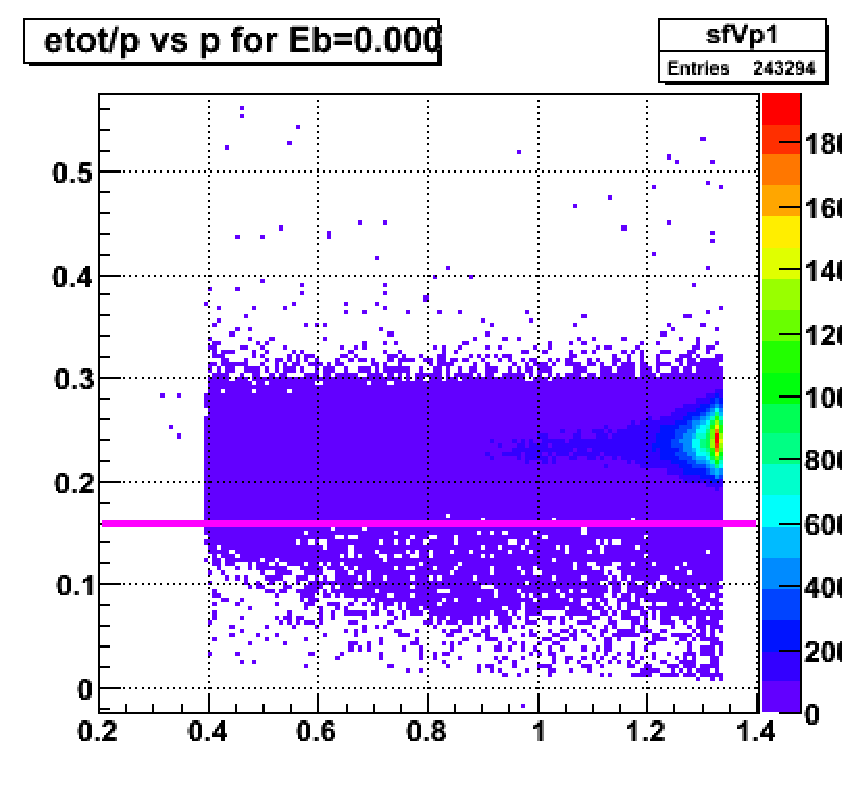
\includegraphics[width=1.0\textwidth]{chap4simul/FigConv/stdECcutsSfvP_Eb1.eps}  %0.6 is the fraction of the real image width????
\centering
%\leavevmode 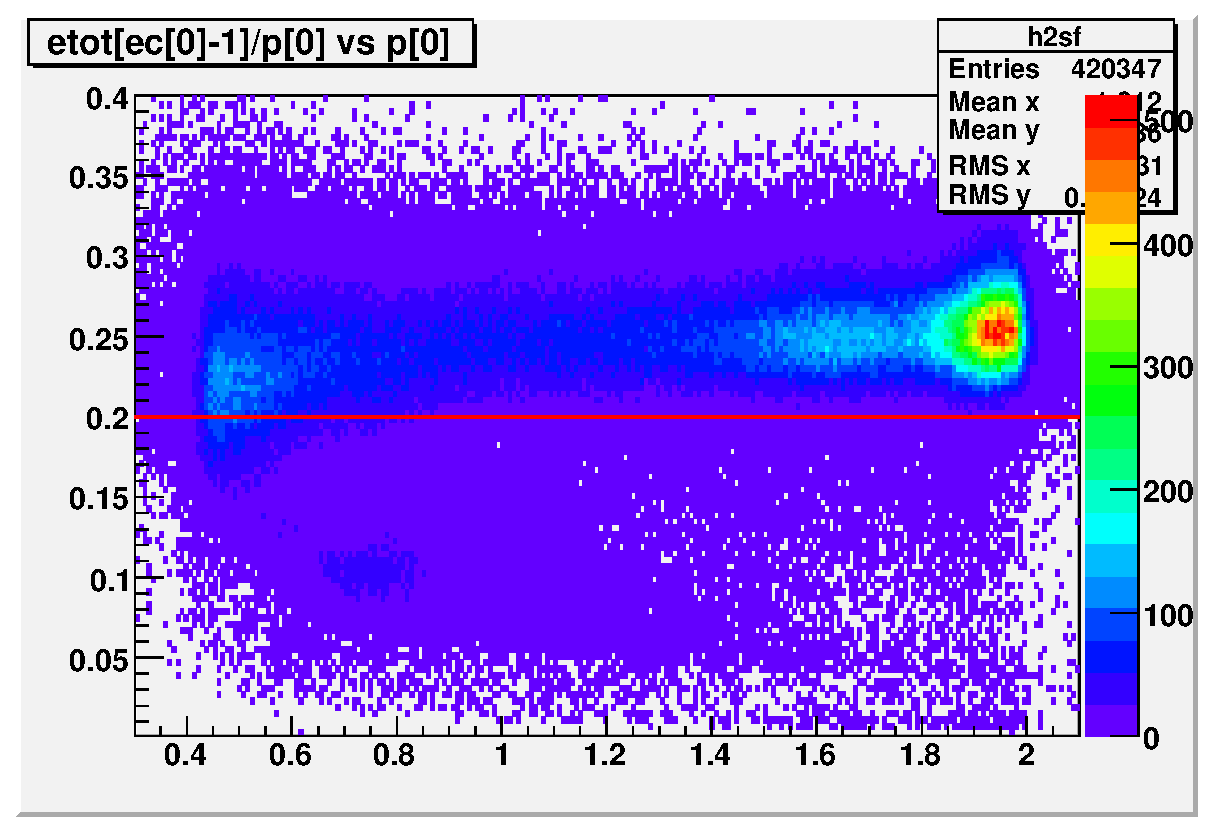
\includegraphics[width=1.0\textwidth]{figuresEG4/FigCuts/ecCuts_sfVp2D_Eb2allEv.eps}  %2.0 GeV data
\leavevmode 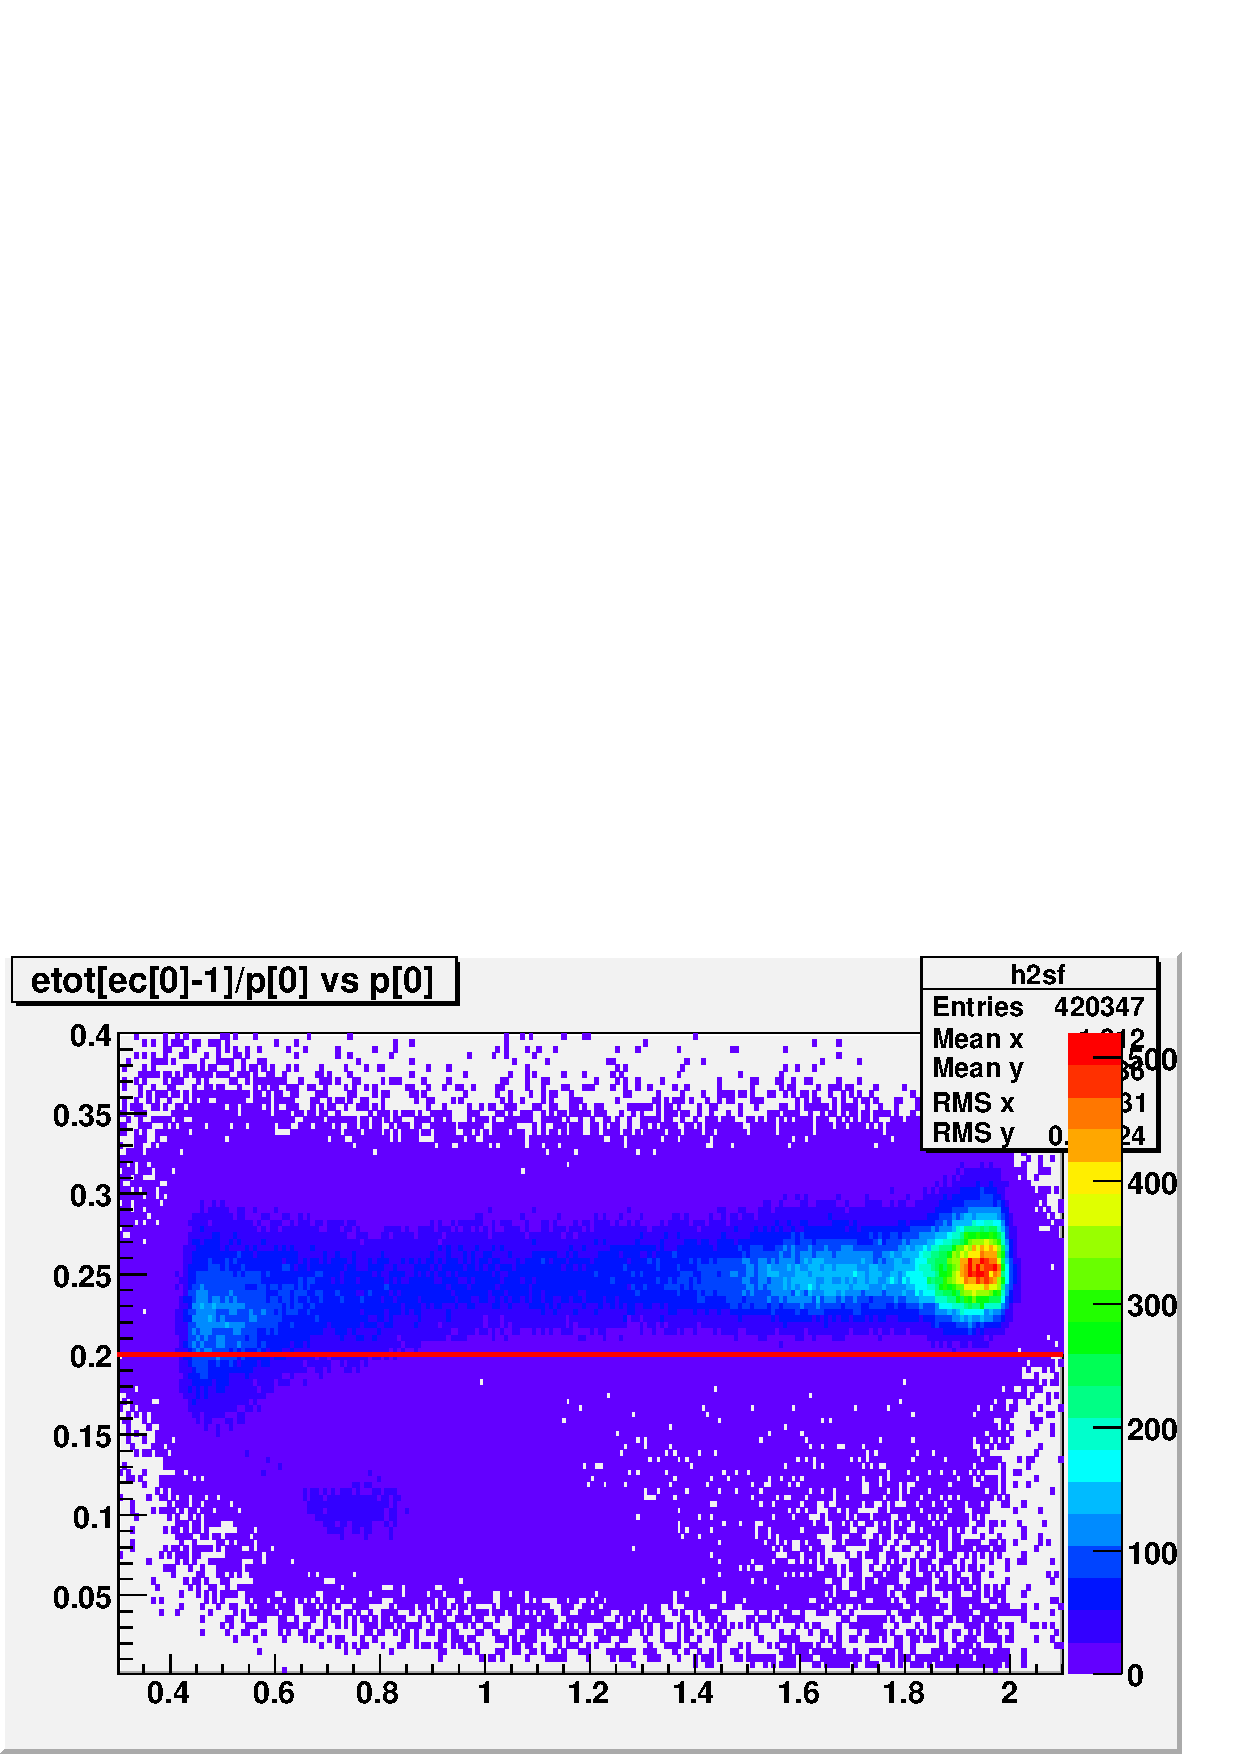
\includegraphics[width=0.8\textwidth]{figuresEG4/FigCuts/ecCuts_sfVp2D_Eb2allEv.png}  %2.0 GeV data
\caption[EC sampling fraction cut (2.0 GeV)]{An example of the cut on the EC sampling fraction (2.0 GeV data). The plots shows the distribution of the sampling fraction (in Y-axis) plotted against the particle momentum (in X-axis). The brighter stripe above about 0.2 in the energy fraction are due to the electrons whereas those below are the pions.
 %\textcolor{red}{SEK: Y-label (Sampling fraction); arrow/or texts indicating pions and electrons. This figure is not very clear - could you use logarithmic z scale? \\ GED: What are the exes? Units? What do we see here?}
}
\label{ecSf}
\end{figure}


%In case of EC in the CLAS, 
For the EC in CLAS, the electron sampling fraction ($etot/p$) is about 0.25 and pions give signals that are mostly below 0.2 (see Fig. \ref{ecSf} or others that follow). Therefore, a lower cut of $etot/p > 0.2$ is usually chosen to reject most of the pions without significantly losing good electrons. However, in %the case of 
our low beam energy experiment, %with its low beam energy, %being relatively smaller, 
few pions are produced and the electron peaks are cleaner in lower kinematic bins as can be seen in the low \qsqs bins of Fig. \ref{ecSfExp6}. Therefore, %in order to have fewer good electrons rejected, 
a \qsqs bin dependent cut of $etot/p > (\mu - 3\sigma)$ was chosen, where $\mu$ and $\sigma$ are the Gaussian fit parameters representing the mean and standard deviation of the distribution in the corresponding \qsqs bin. 
The choice of $3 \sigma$ was decided by looking at the sampling fraction distributions in each of the \qsqs bins and making sure that no pion signal was observed in any of the bins.


On simulated data also, a corresponding $3 \sigma$ cut was applied by first repeating the exact same procedure to get the corresponding values of $\mu$ and $\sigma$ from the simulated data. Using same-$\sigma$ cuts %(i.e. the same relative distance from the electron peaks) 
in corresponding \qsqs bins of both experimental and simulated data ensures that we had the same fraction of data in corresponding bins from both experimental and simulated sides. 



\begin{figure}[H]%[htp] %ht, htpb (p - float, b = bottom, h=? t = top)
\centering
%\leavevmode 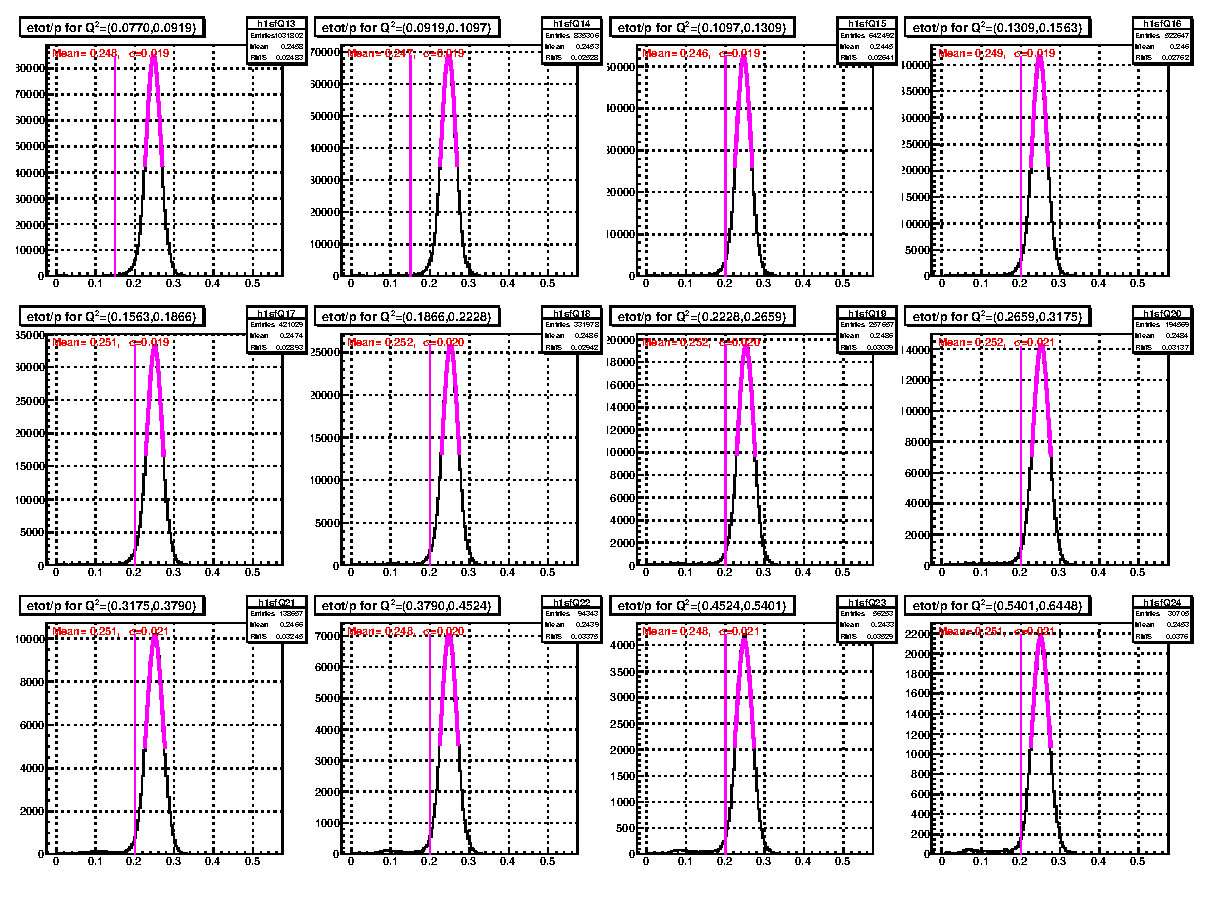
\includegraphics[width=1.0\textwidth]{chap4simul/FigCuts/ecCuts_sfOneD_Eb2_4Th.eps}  %0.6 is the fraction of the real image width????
%\leavevmode 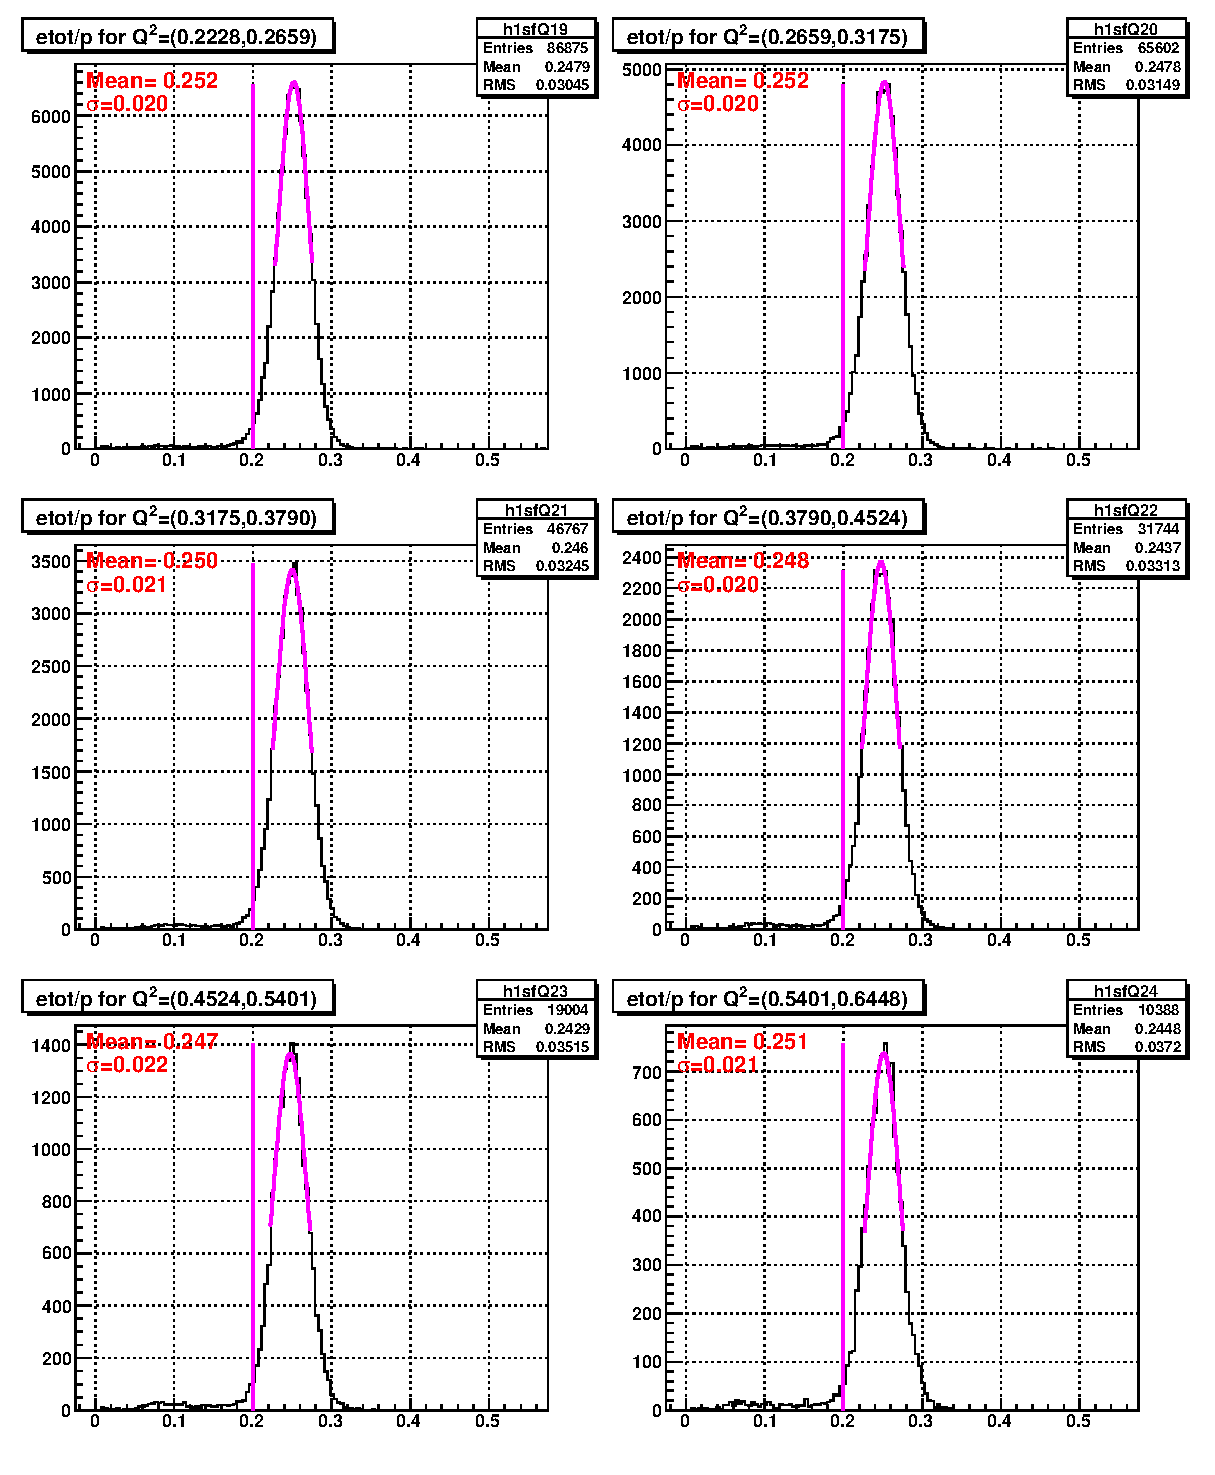
\includegraphics[width=1.0\textwidth]{chap4simul/FigCuts/ecCuts_sfOneD_Eb2_4ThN.eps}  %0.6 is the fraction of the real image width????
\leavevmode 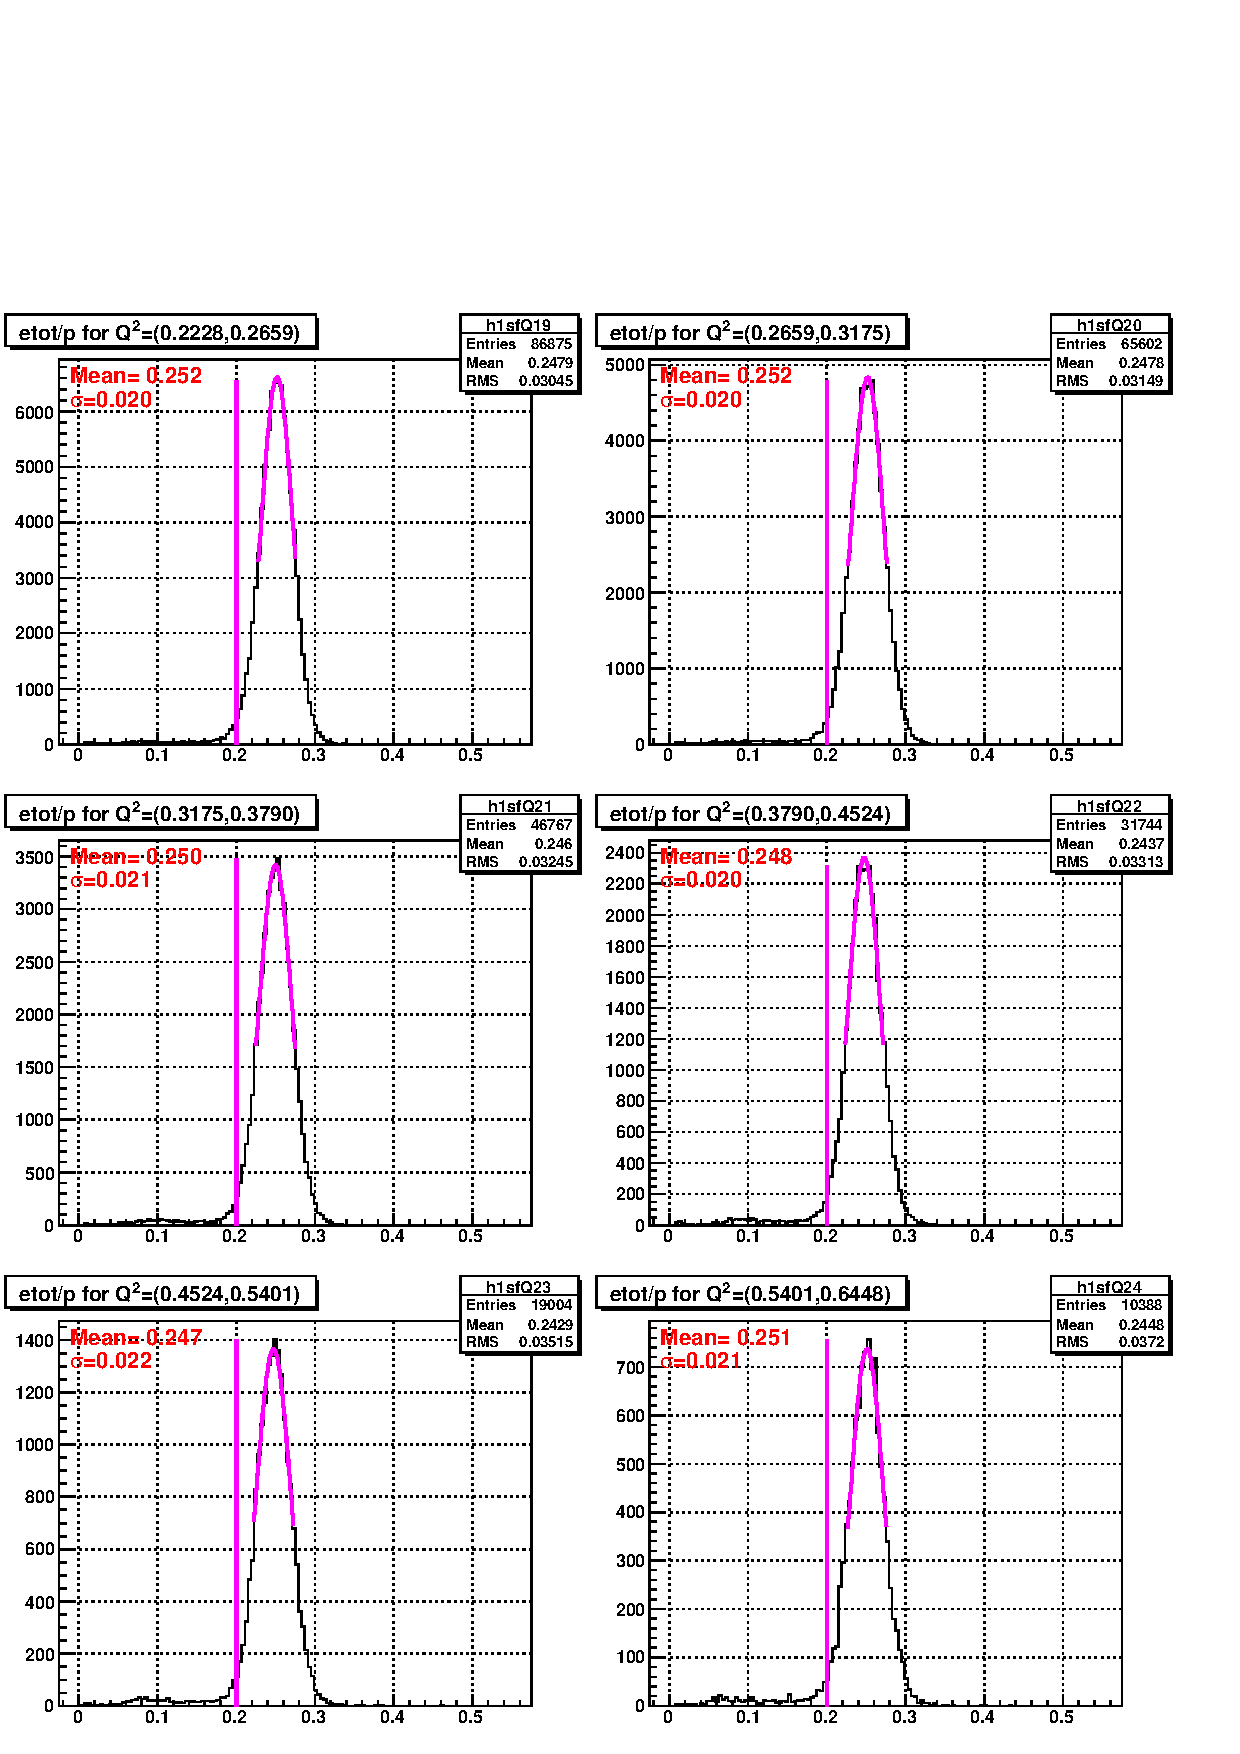
\includegraphics[width=1.0\textwidth]{figuresEG4/FigCuts/ecCuts_sfOneD_Eb2_4ThN.png}  %0.6 is the fraction of the real image width????
\caption[EC sampling fraction cut (Exp.)]{The \qsqs dependent cuts on the EC sampling fraction for 2.0 GeV experimental data. Events below the red lines are rejected.}
\label{ecSfExp6}
\end{figure}



\begin{figure}[H]%[htp] %ht, htpb (p - float, b = bottom, h=? t = top)
\centering
%\leavevmode 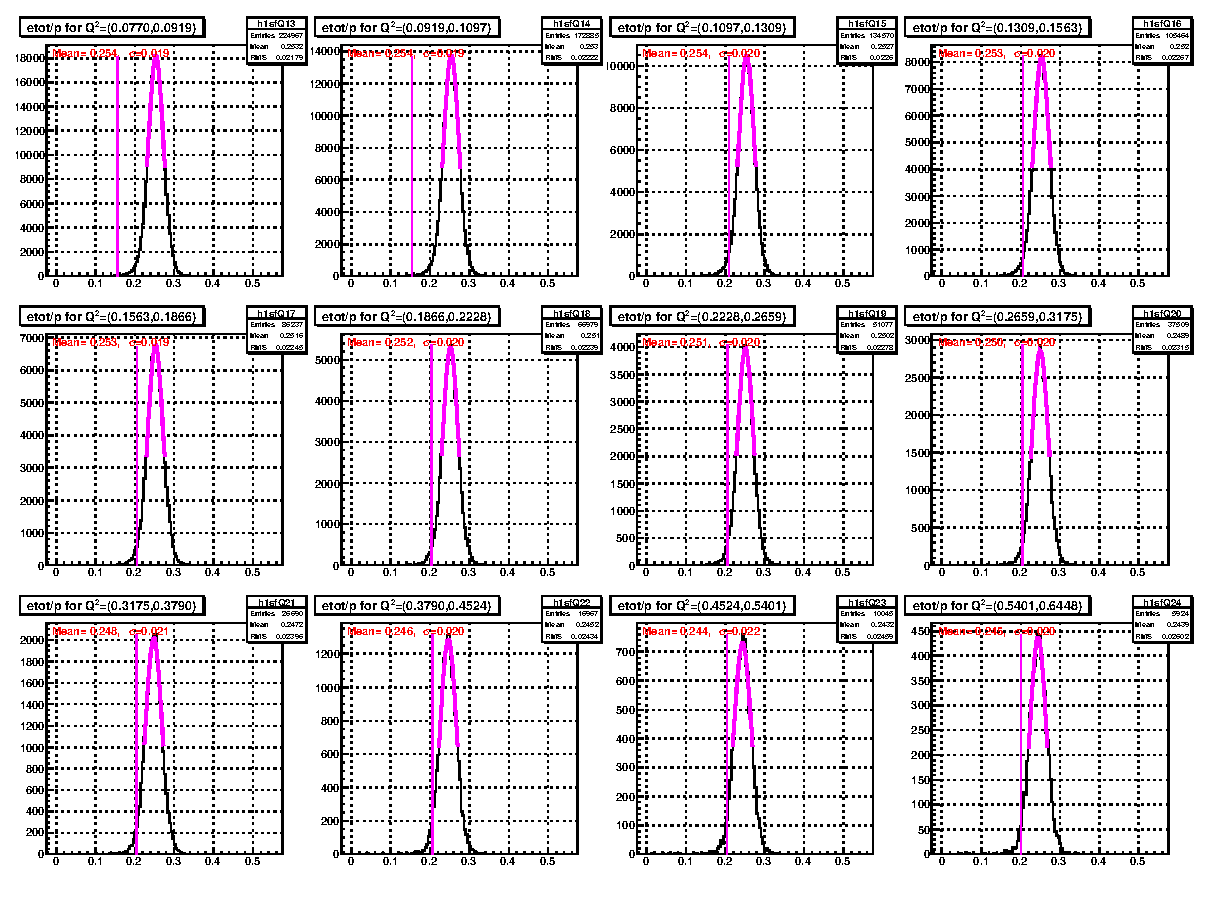
\includegraphics[width=1.0\textwidth]{chap4simul/FigCuts/ecCuts_sfOneD_Eb2_4Thsim.eps}  %0.6 is the fraction of the real image width????
%\leavevmode 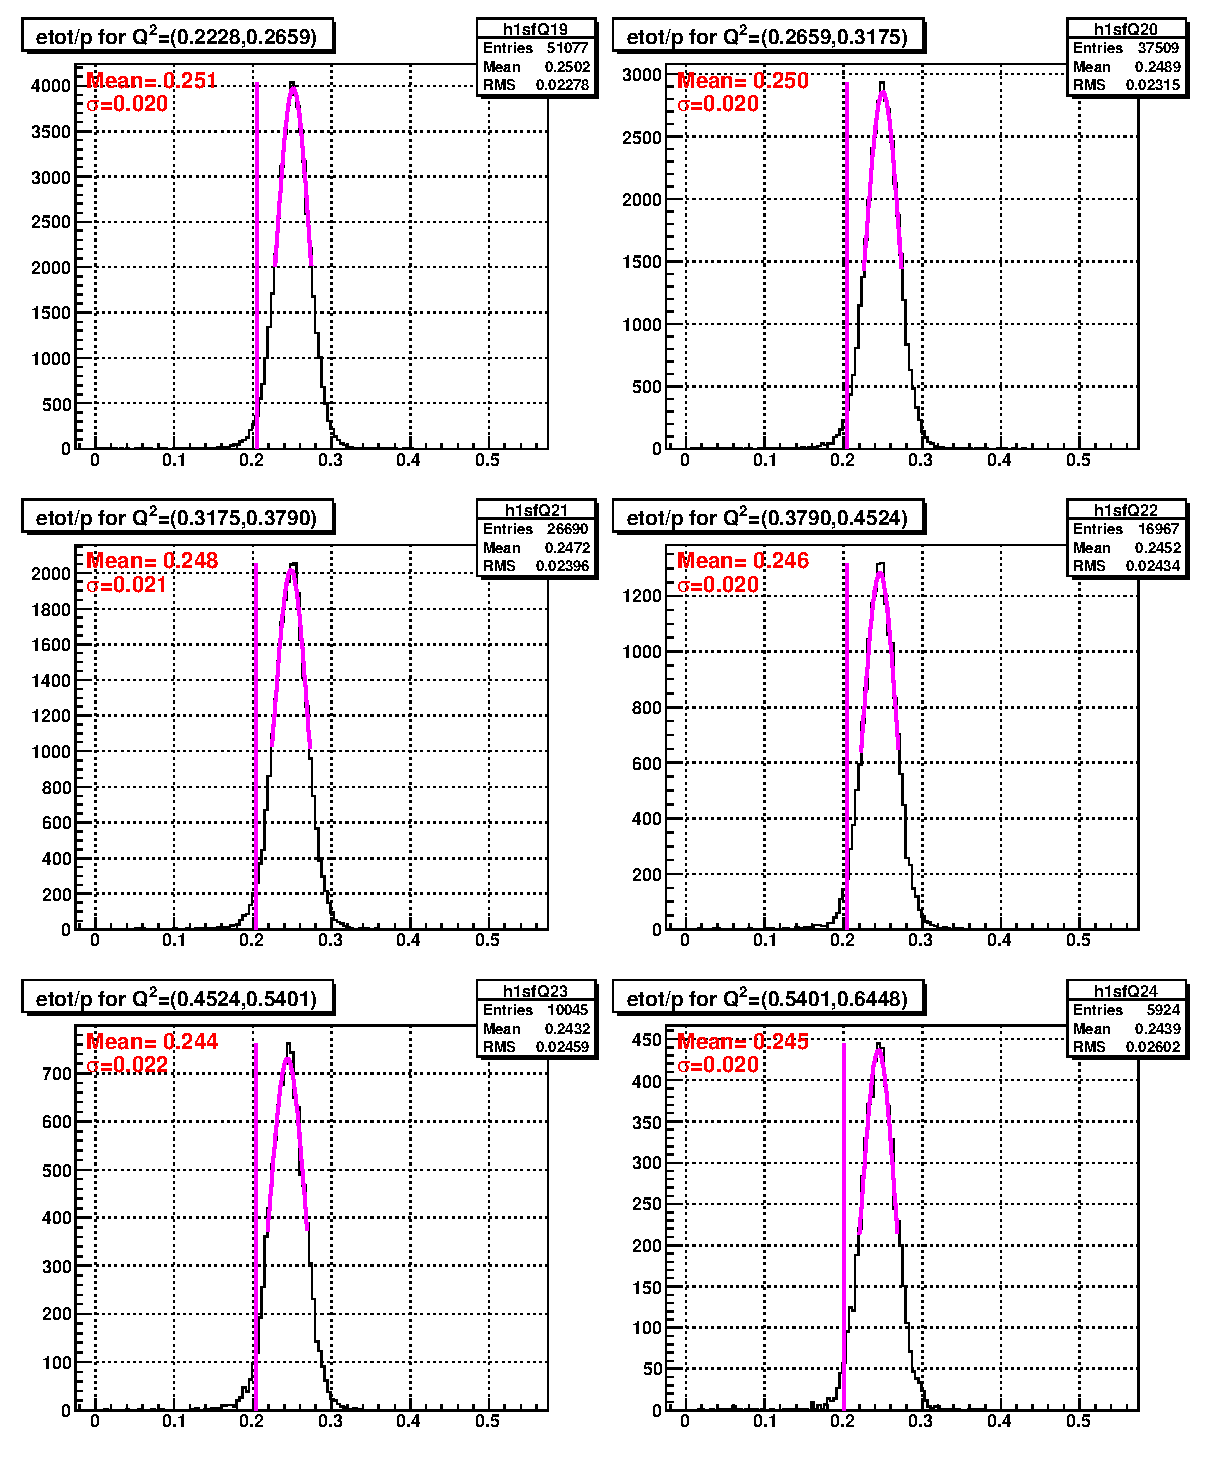
\includegraphics[width=1.0\textwidth]{chap4simul/FigCuts/ecCuts_sfOneD_Eb2_4ThsimN.eps}  %0.6 is the fraction of the real image width????
\leavevmode 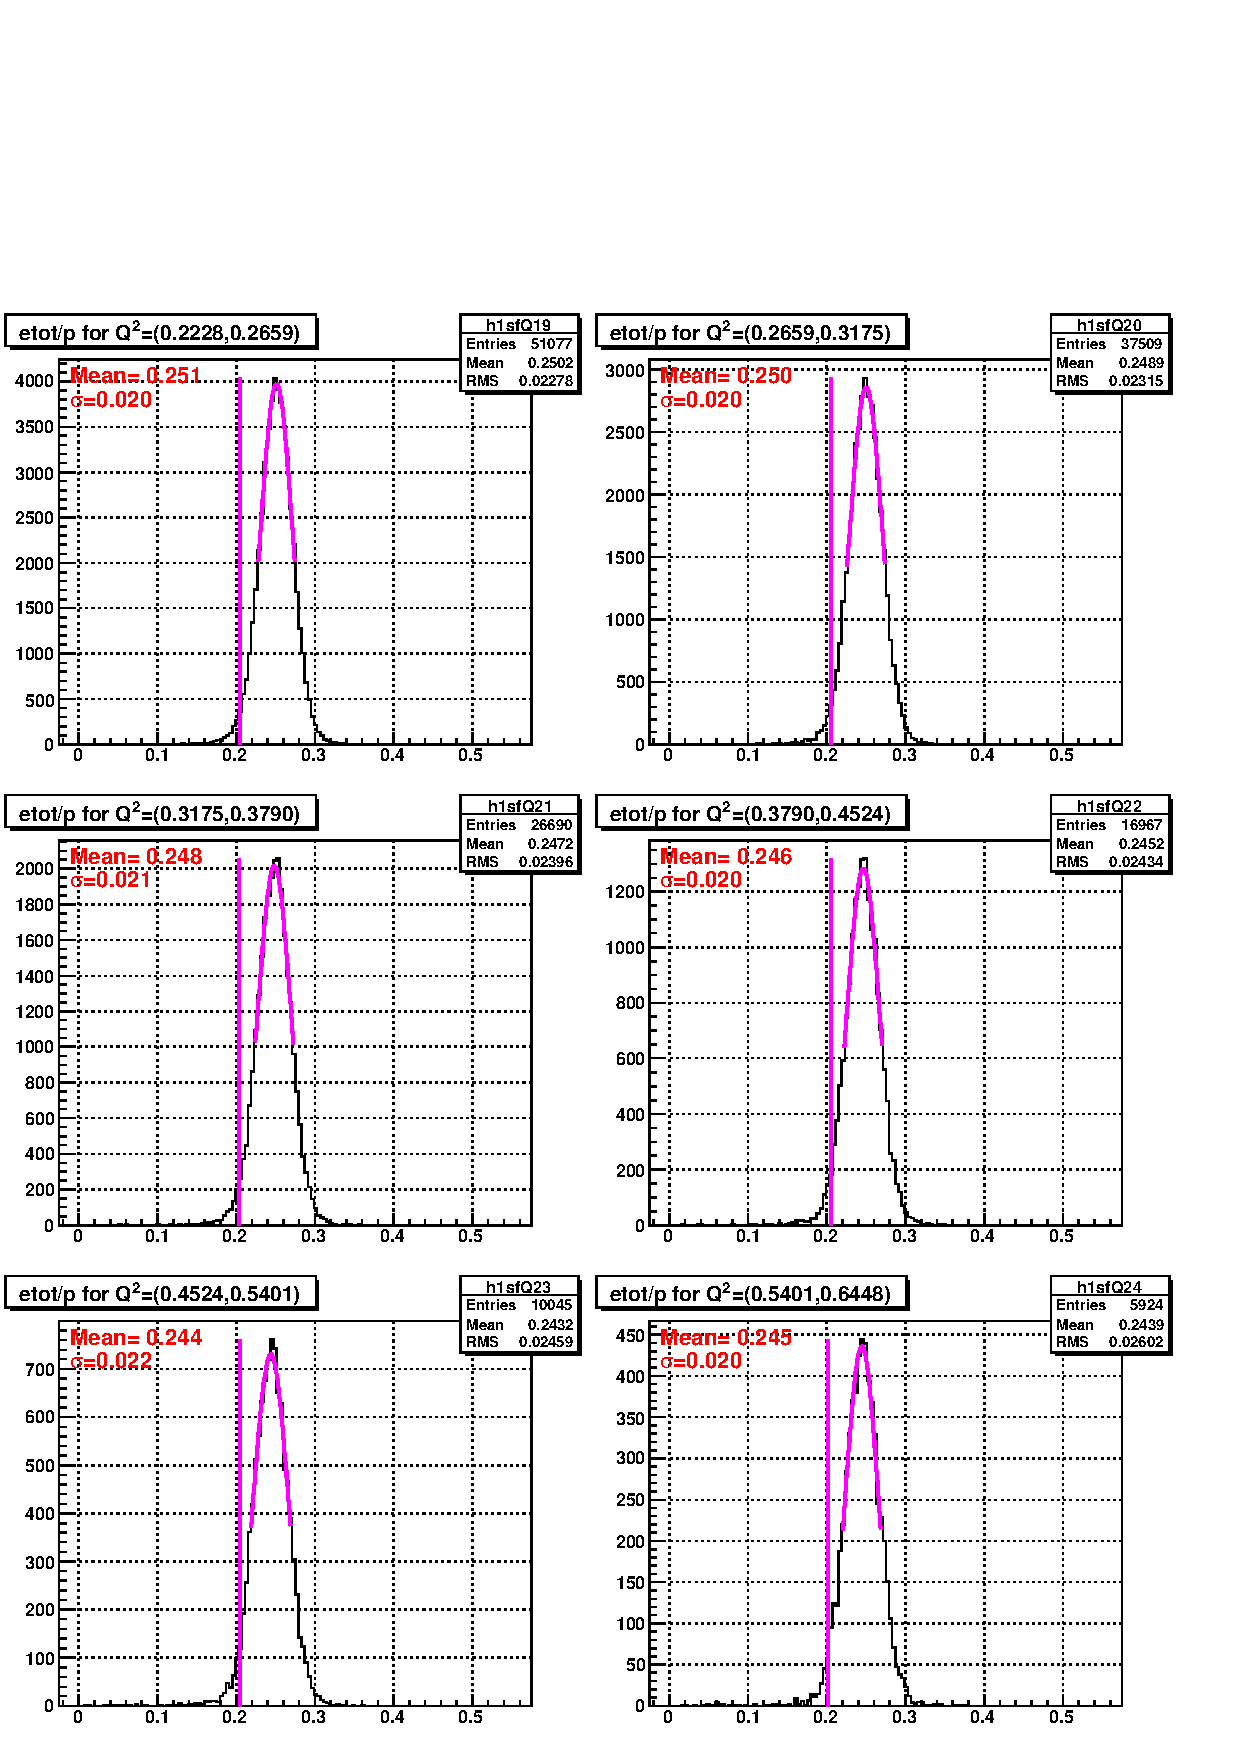
\includegraphics[width=1.0\textwidth]{figuresEG4/FigCuts/ecCuts_sfOneD_Eb2_4ThsimN.png}  %0.6 is the fraction of the real image width????
\caption[EC sampling fraction cut (Sim.)]{The \qsqs dependent cuts on the EC sampling fraction for 2.0 GeV simulation data. Events below the red lines are rejected.}
\label{ecSfSim6}
\end{figure}


%In short, only two numbers 0.15 and 0.2 define the cuts on the experimental data, but the cuts for simulation data are all different, yet they are at the same relative distance from the electron peaks as in the experimental data and, therefore, include about the same fraction of good electrons. 

%\textbf{\textcolor{red}{This section may have been too verbose and complex to understand.}}
% http://en.wikipedia.org/wiki/Particle_shower:   An ``electromagnetic shower'' begins when a high-energy electron, positron or photon enters a material. At high energies (above a few MeV, below which photoelectric effect and Compton scattering are dominant), photons interact with matter primarily via pair production  that is, they convert into an electron-positron pair, interacting with an atomic nucleus or electron in order to conserve momentum. High-energy electrons and positrons primarily emit photons, a process called bremsstrahlung. These two processes (pair production and bremsstrahlung) continues until photons fall below the pair production threshold, and energy losses of electrons other than bremsstrahlung start to dominate. 
%In the case of experimental data, the sampling fraction is cut at 0.2 in the first fourteen \qsqs bins and at 0.15 in the others. But, in the case of simulated data, the cuts are variable, but still are correlated with the cuts on the real data. To ensure the proportional/same fraction of events from both real and simulated data in a given \qsqs bin, the electron peaks on those data are first fitted to Gaussian distributions to find the peak position and width (represented by $\sigma$ i.e. the standard deviation), and then cut position on simulated data is determined by the value which is at the same distance from  the average in terms of $\sigma_{sim}$ as the cut on real data is from its own mean in terms of $\sigma_{exp}$.






\subsubsection{Cuts on $E_{in}$}
\begin{figure}[h] %ht, htpb (p - float, b = bottom, h=? t = top)
\centering
%\leavevmode 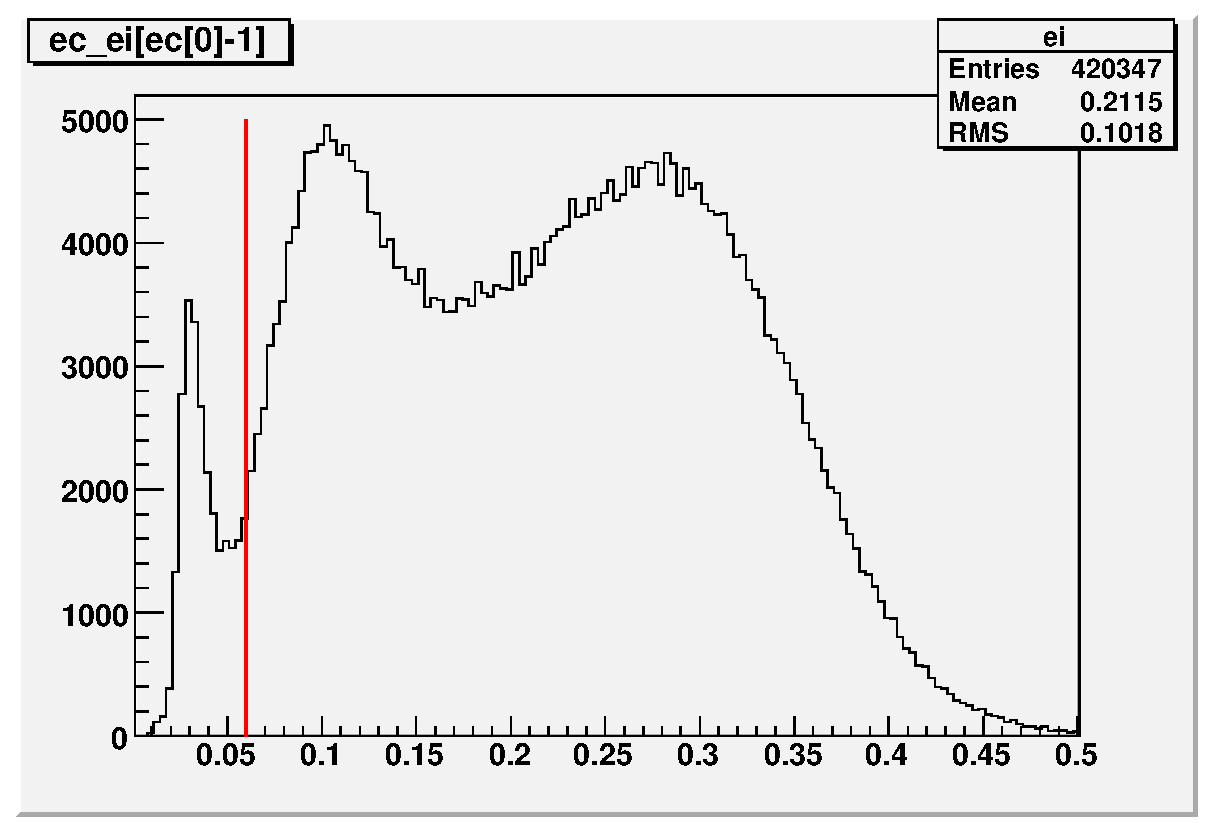
\includegraphics[width=0.8\textwidth]{chap4simul/FigCuts/ec_eiCutFrmRtPrmtClasEb2.eps}  %0.6 is the fraction of the real image width????
\leavevmode 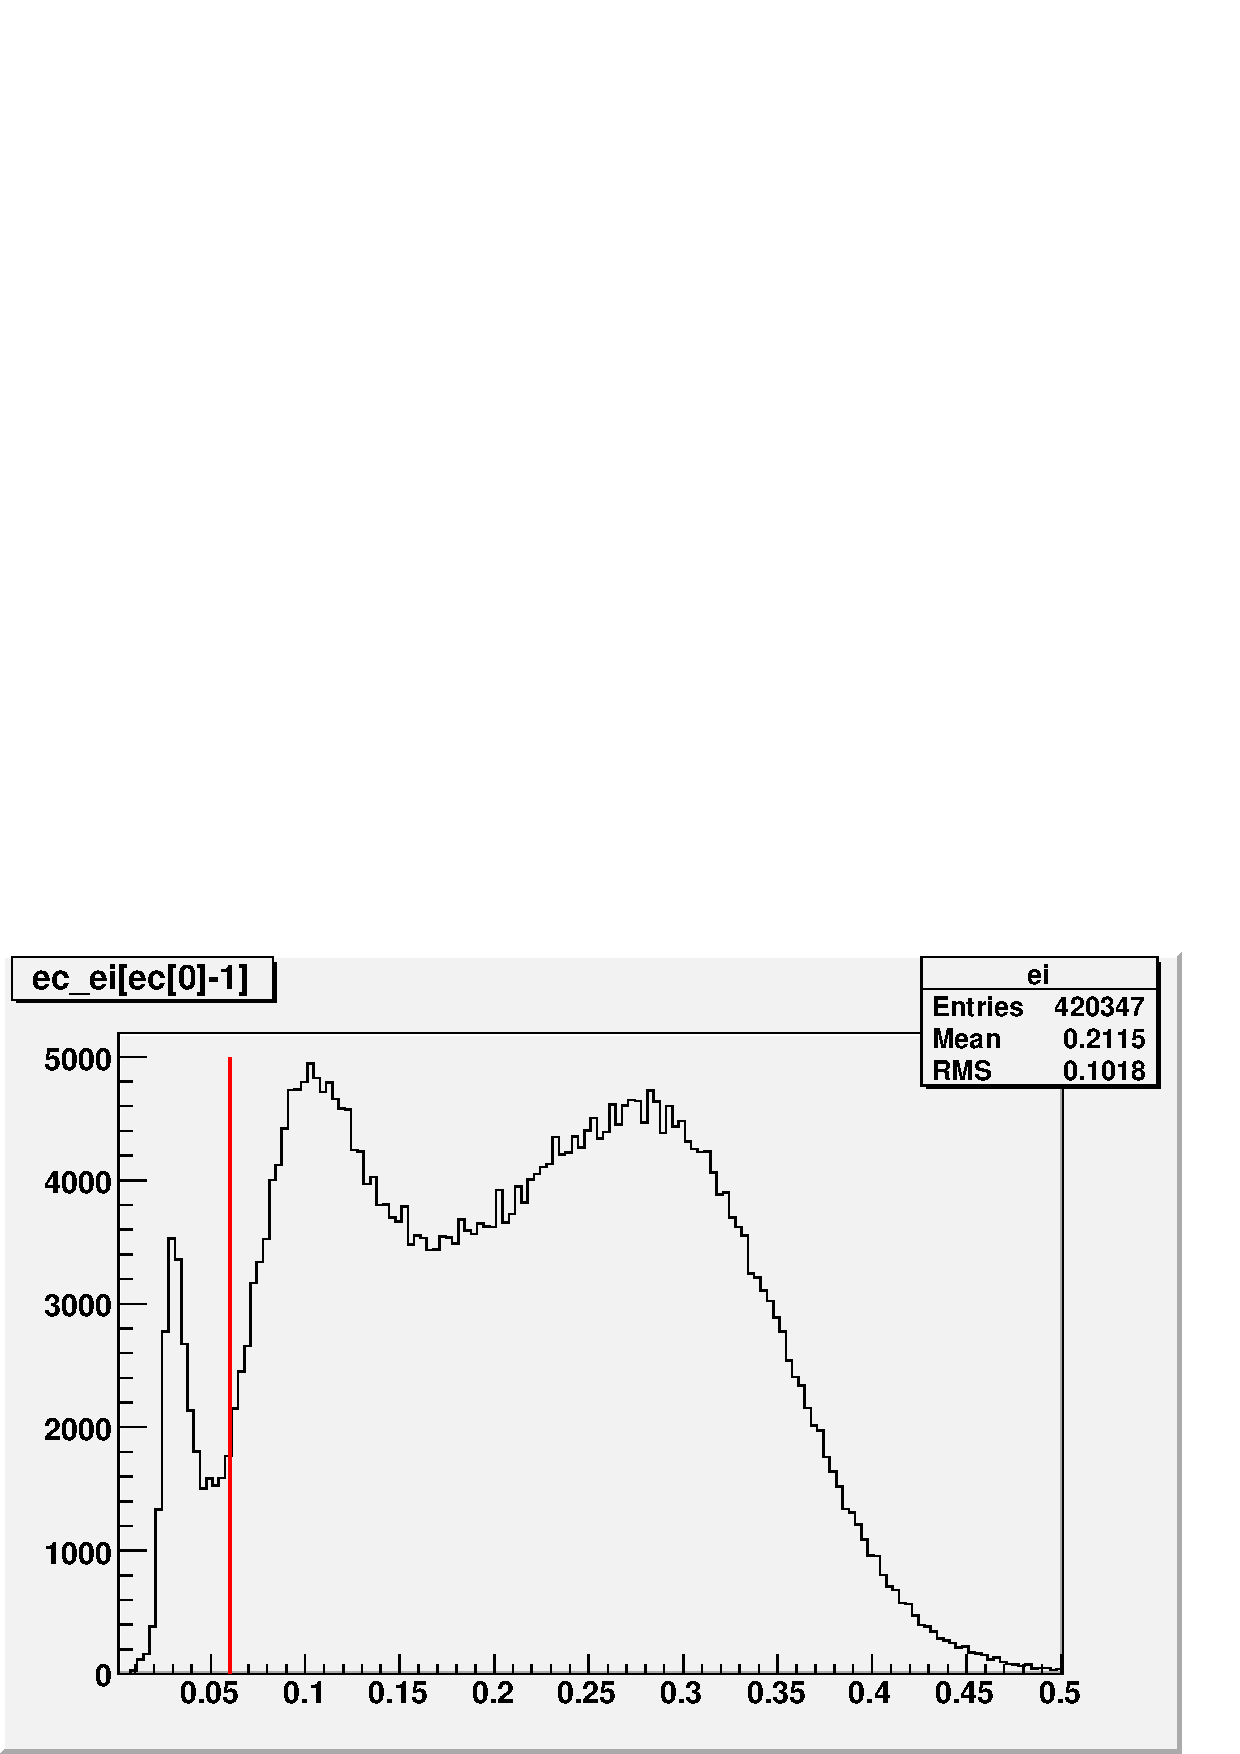
\includegraphics[width=0.8\textwidth]{figuresEG4/FigCuts/ec_eiCutFrmRtPrmtClasEb2.png}  %0.6 is the fraction of the real image width????
\caption[EC inner energy cut (2.0 GeV)]{Energy deposited (GeV) in the inner EC and the cut (red line) used to reject pions (seen as a peak at about 0.03 GeV) from a sample of electron candidates of 2.0 GeV data.}
\label{ecInExp1}
\end{figure}

Pions, which do not shower and are minimum ionizing particles in the momentum range detected in CLAS, deposit only a small amount of energy in the inner part of the EC, %in the ratio of about 5:3, independent on their momentum. %https://userweb.jlab.org/~ungaro/maureepage/proj/pi0/e_pid/note/electron_pid.html#x1-100001.7
independent of their momentum. When $E_{in}$ is histogrammed, the small pion signal peak at about 0.03 clearly stands out from the large electron sample, with little overlap in between. So, a universal cut of $E_{in}$=0.05 on both data and simulation (as shown in Figs. \ref{ecInExp1}, \ref{ecInExp6} and \ref{ecInSim6}) safely rejects most of the pions from the electron candidate sample. 


\begin{figure}[H]%[hp] %ht, htpb (p - float, b = bottom, h=? t = top)
\centering
%\leavevmode 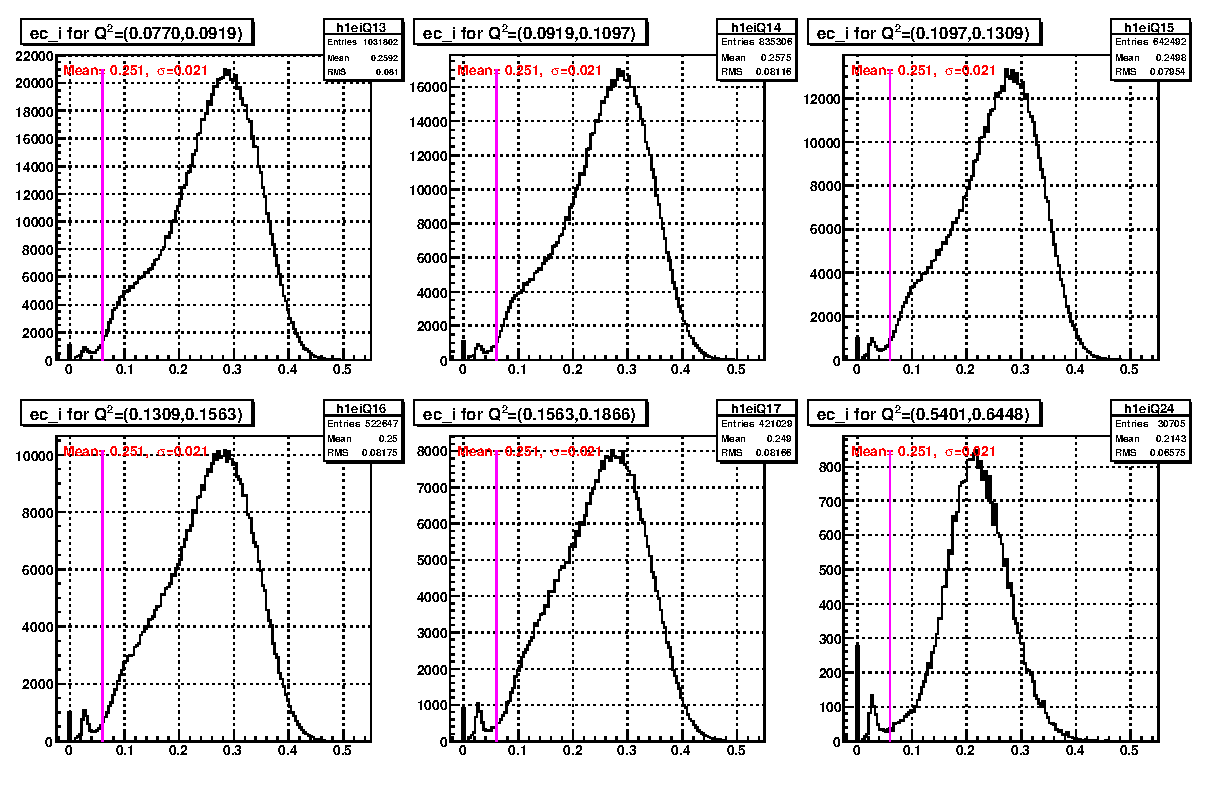
\includegraphics[width=1.0\textwidth]{chap4simul/FigCuts/ecCuts_eiOneD_Eb2_4Th.eps}  %0.6 is the fraction of the real image width????
\leavevmode 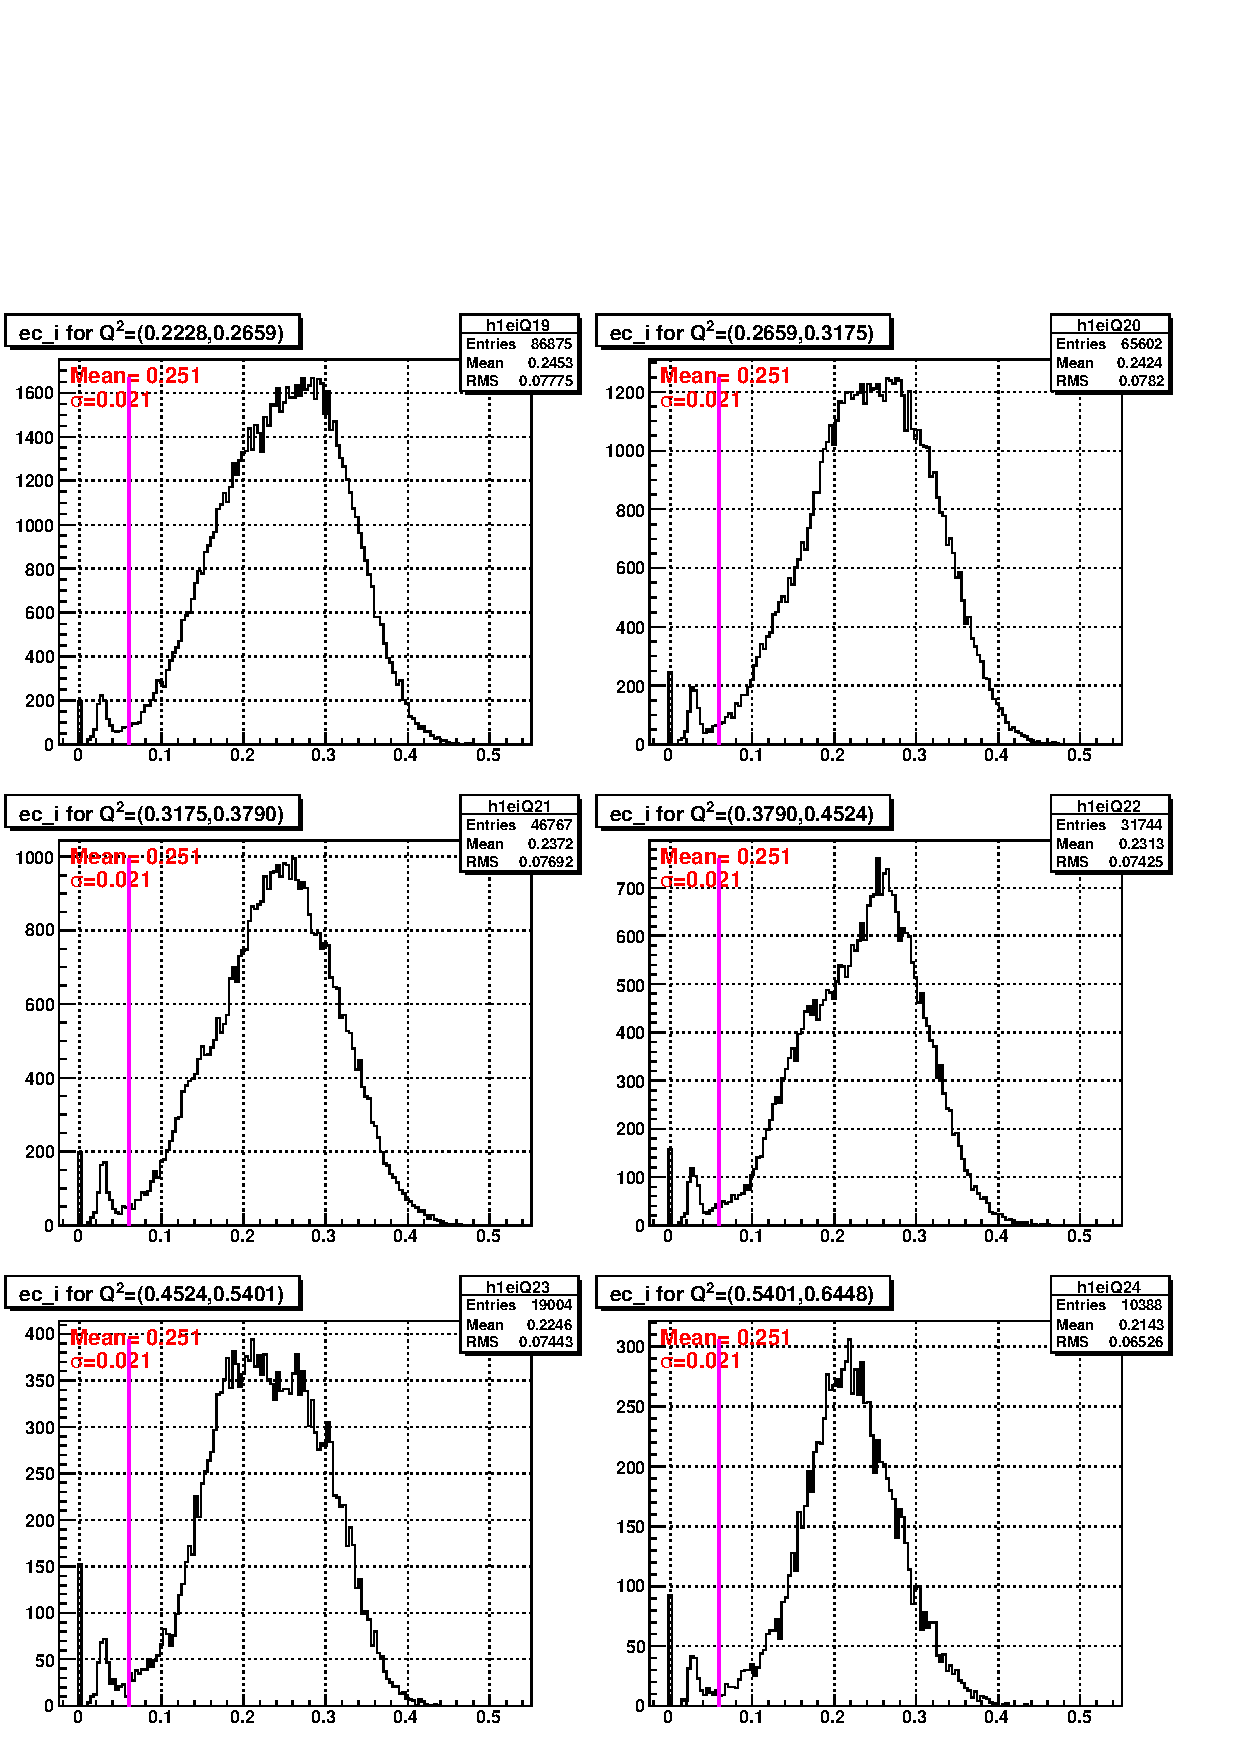
\includegraphics[width=1.0\textwidth]{figuresEG4/FigCuts/ecCuts_eiOneD_Eb2_4ThN.png}  %0.6 is the fraction of the real image width????
\caption[EC inner energy cut (Exp.)]{The EC-inner cut on a sample of 2.0 GeV experimental data in various \qsqs bins.}
\label{ecInExp6}
\end{figure}



\begin{figure}[H]%[hp] %ht, htpb (p - float, b = bottom, h=? t = top)
\centering
\leavevmode 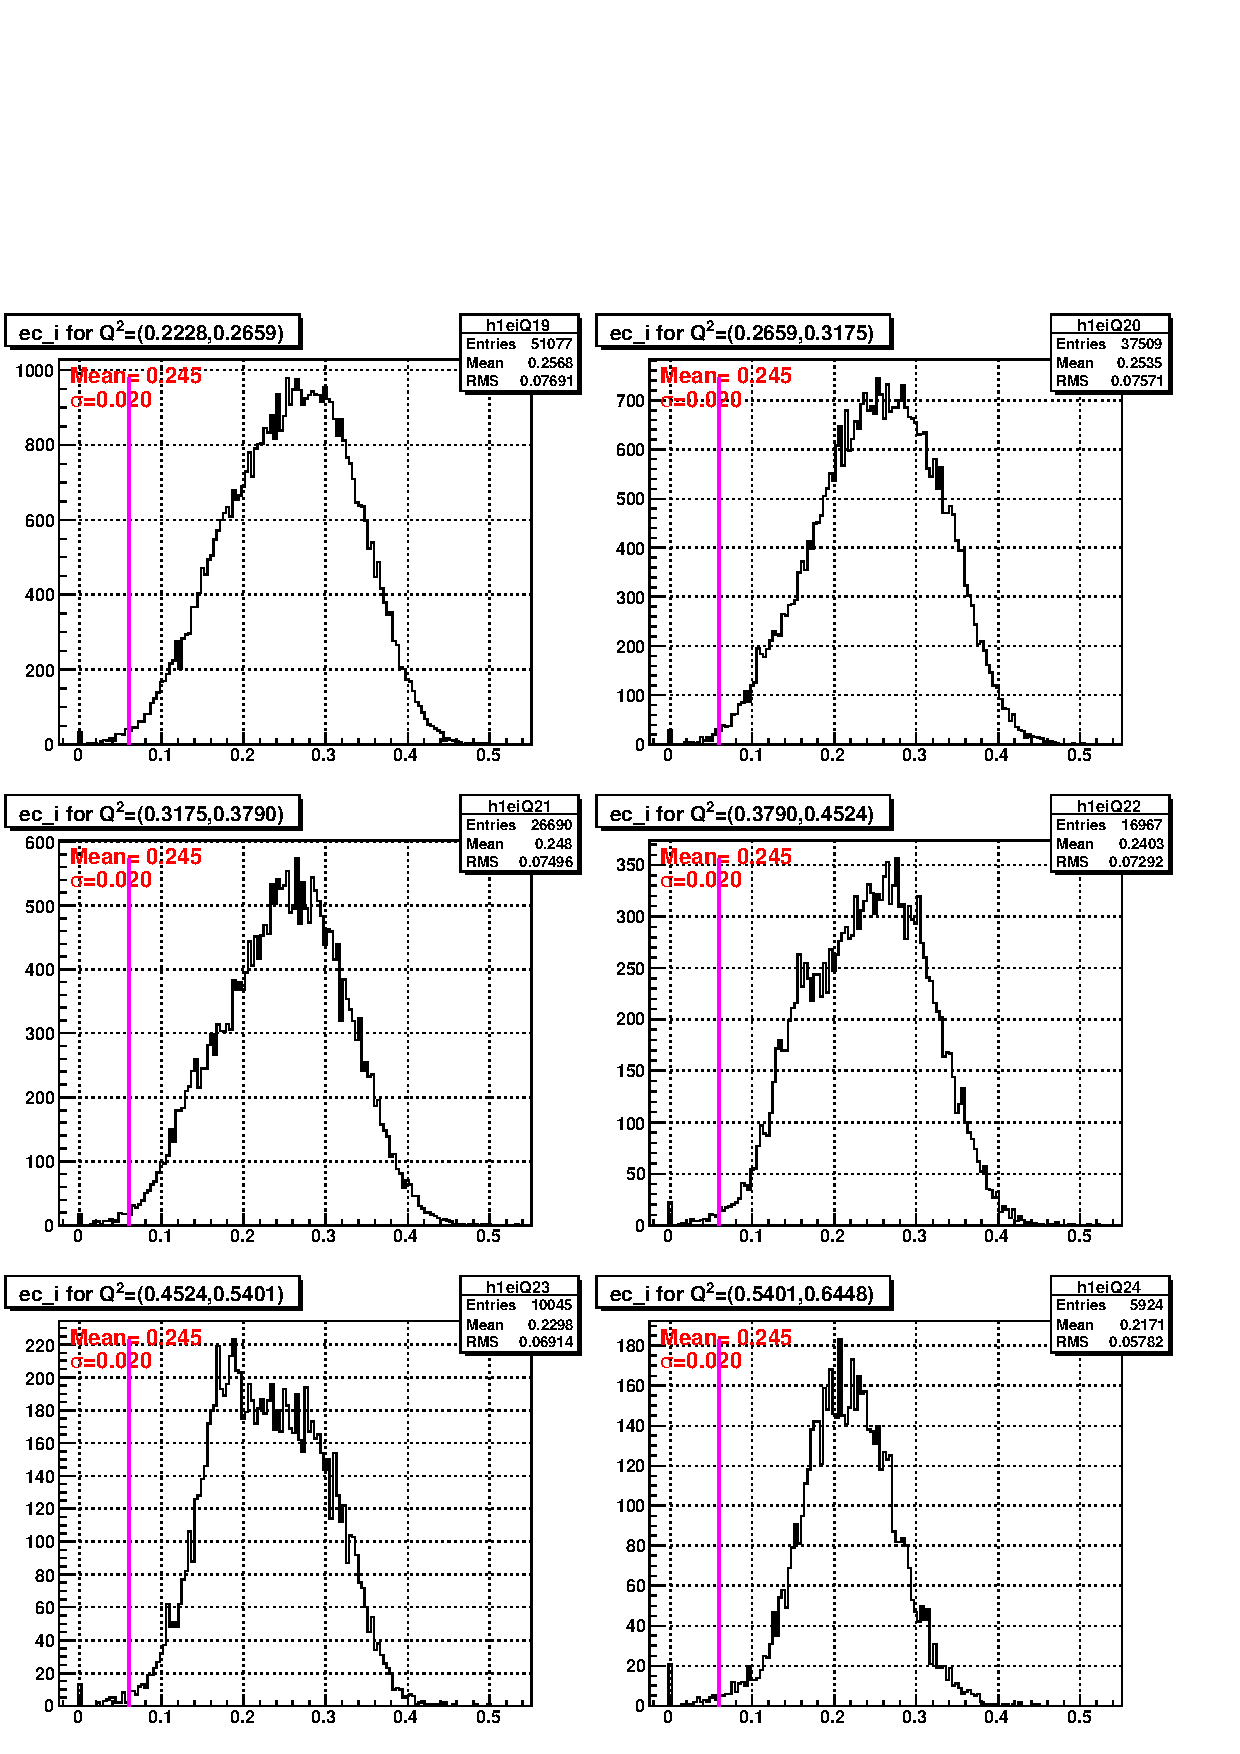
\includegraphics[width=1.0\textwidth]{figuresEG4/FigCuts/ecCuts_eiOneD_Eb2_4ThsimN.png}  %0.6 is the fraction of the real image width????
\caption[EC inner energy cut (Sim.)]{The EC-inner cut on a sample of 2.0 GeV simulation data in various \qsqs bins.}
\label{ecInSim6}
\end{figure}




\begin{comment} %Part copied from my thesis (just to remind myself what I had done)

\subsubsection{Cuts on $E_{out}$}
In addition to the two EC-cuts above, one more cut based on the correlation between EC-outer and EC-inner %ec\_o/p and ec\_i/p 
(as shown in Fig. \ref{ecOvI}) was used which helps further to clean up the electron sample. %pion contamination. %%%SEK cor.

\begin{figure}[H]%[h] %ht, htpb (p - float, b = bottom, h=? t = top)
\centering
\leavevmode 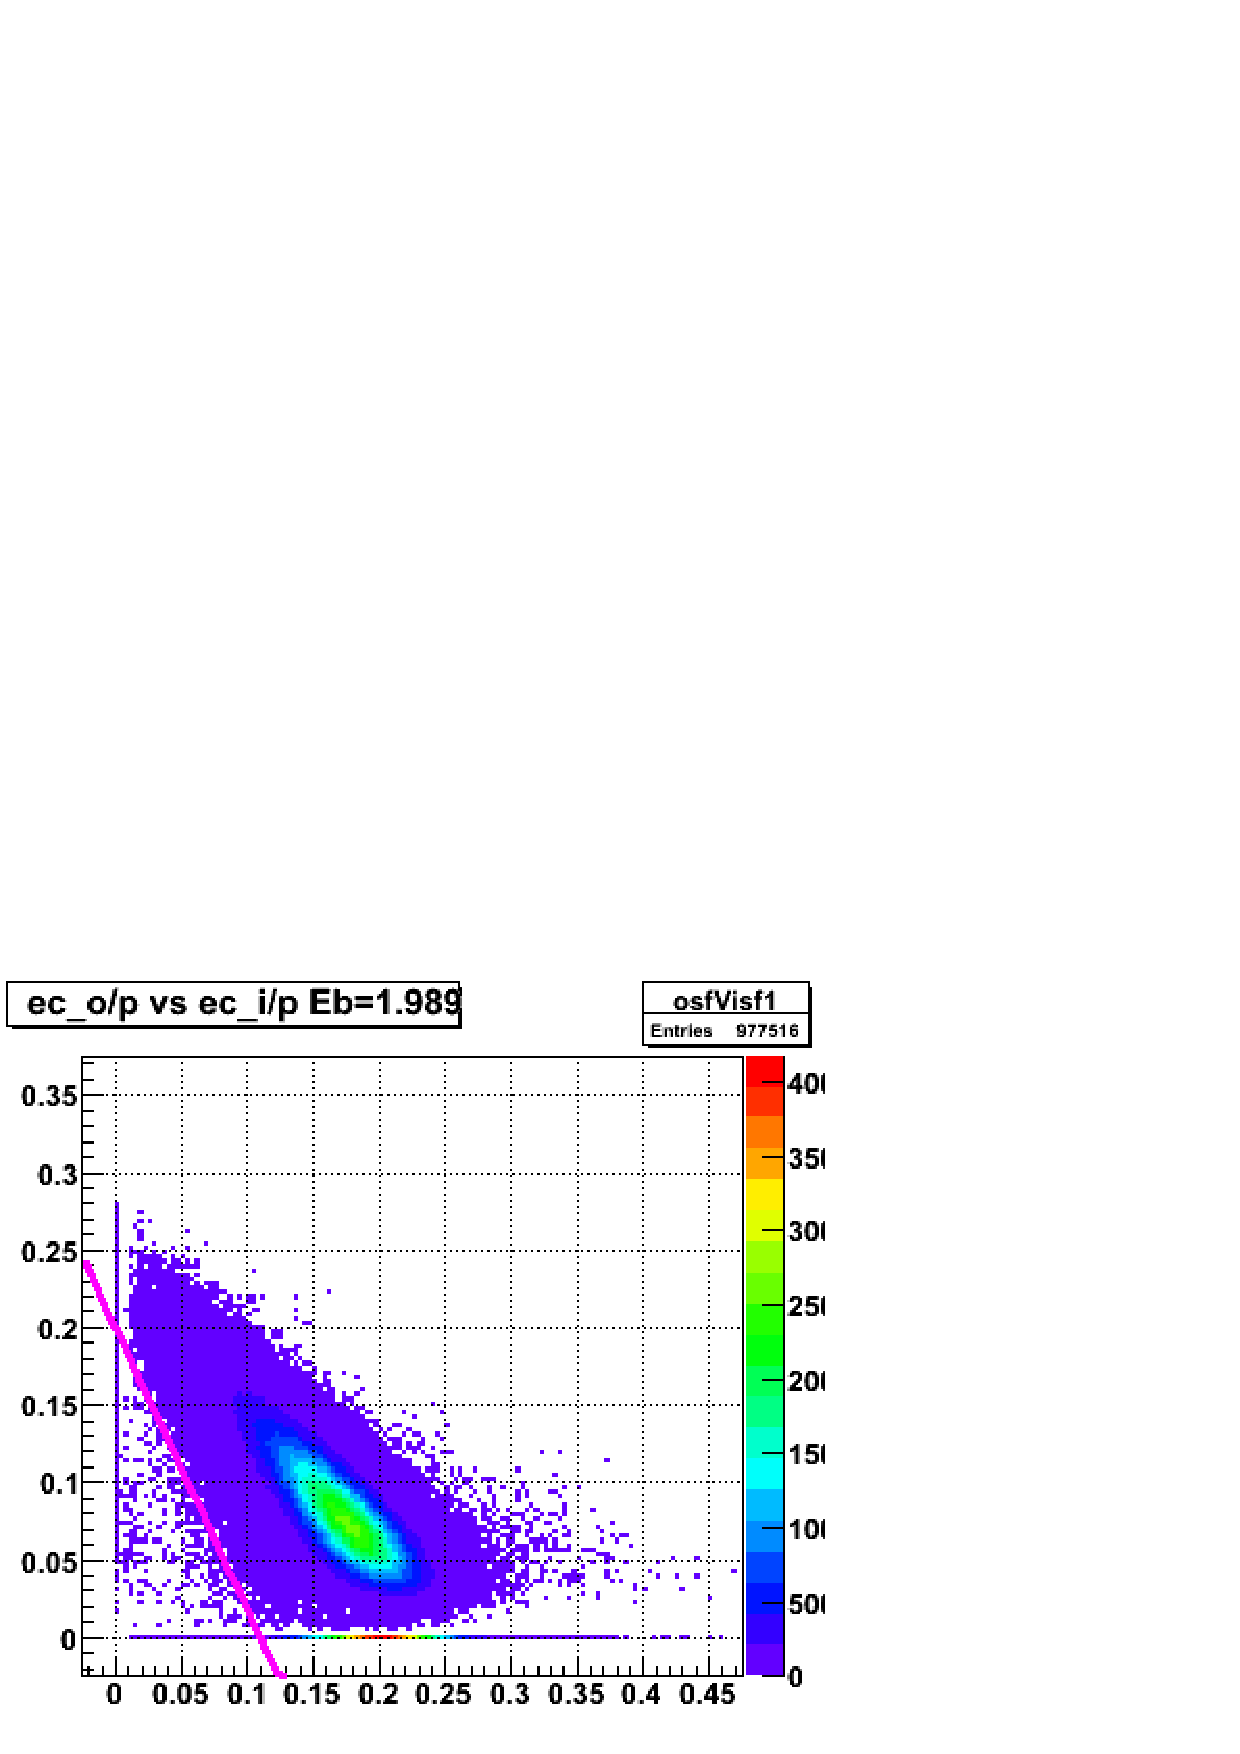
\includegraphics[width=0.8\textwidth]{figuresEG4/FigConv/stdECcutsSfovSfi_Eb2sim.png}  %0.6 is the fraction of the real image width????
\caption[EC inner and outer energy cut (Exp.)]{Energy detected in EC outer as a function of EC inner, both normalized with the particle momentum, for the 2 GeV data. The brown line shows the EC cut to reject pions (which fall below that line).}
\label{ecOvI}
\end{figure}

\end{comment}

\subsection{Cerenkov Counter Cuts}
\subsubsection{ Osipenko (CC Geometry and Time Matching) Cuts}
\label{osiCuts}
As discussed in Sec. \ref{cha:EG4} %{expSetUp} %Or refer directly to the CC section (by its own label, to be added)  (There were 18 modules in the old CC of of each CLAS sector)
the new EG4-dedicated CC consists of 11 modules %/segments 
each consisting of a pair %each 
of mirrors and PMTs. The segments are placed along the CLAS polar angle covering 15 to 45 degrees, i.e., the segments are at different polar angular positions. % See presentation cerenkov_son_july2003 (in the UbuntuOne/EG4nMore1/Jlab/Detector/CLASdetector/CC (also have a look at other presentations as well as E. Golovach's work on the Cerenkov (linked from EG4 wiki main page - http://www.ge.infn.it/~golovach/cerenkov/ (I can/may find a lot of plots and design diagrams))
During normal operation, the PMTs of these segments may produce %a certain amount of noise signal 
thermal noise that is equivalent to that produced by one photo-electron passing through it. As a result, when a noise pulse in the CC and a pion track measured by DC coincides within the trigger window of the CLAS detector, %Nevzat writes the window is 150 ns; thesis pg 145
the track gets registered as an electron candidate by the event reconstruction program, thus contributing to the contamination of electron candidates % samples 
with the misidentified pion tracks. In fact, this turns out to be the biggest source of pion contamination. In order to minimize such contamination and help better identify electrons from pions, %the 
CC geometric and time-matching cuts are applied.

%https://userweb.jlab.org/~ungaro/maureepage/proj/pi0/e_pid/note/electron_pid.html#x1-120001.9
%The cuts in this category
This category of cuts for this experiment is %by X. Zheng \cite{eg4wiki} - one of the collaborators of the experiment. Her work, in turn, was 
mostly based on a similar analysis done for another CLAS experiment by M. Osipenko \cite{cnOsipenko, anaNoteXZheng}.% in order to study the CC response and thereby develop a method to better discriminate electrons from pions. 


The first requirement in the CC-matching is for the electron candidate track (as reconstructed by DC) to have a corresponding signal in CC. In addition, the track needs to meet several %the following %GED
matching conditions to be acceptable as described in the next sections.


%\subsubsubsection{CC \th Matching} %http://tex.stackexchange.com/questions/186981/is-there-a-subsubsubsection-command
\paragraph{CC \th Matching}
As said above, the CC segments are at different average polar angle positions (between 15 and 45 degrees), so in principle, one can expect a one-to-one correspondence between the polar angle of the track (as measured at the vertex) and the CC-segment. However, the torus magnetic field bends the particles towards or away from the beamline, so it's more convenient to use the CC projected polar angle \thp  rather than the vertex angle $\theta$, where \thp is defined as the polar angle of the position vector defined by the point of intersection of the track with %the CC plane
the plane at which the CC PMTs reside as reflected by the CC mirrors %xz: I think instead of "the CC plane" you should say "the plane at which the CC PMTs reside as reflected by the CC mirrors."
(another projected angle \php is the azimuthal angle of the same vector). These projected angles can be uniquely calculated for each track based on the DC %and CC 
signals of the track as well as the CC geometry information. To simplify the later analysis process, these projected angles for each track were calcuated during the final %/pass1 version  of the
 data reconstruction process and then saved in the output files %(in ntuple-10 format)
  just like all the other %usual 
 information for the events and particles. 
Finally, for the actual electrons a one-to-one correspondence between \thp and the segment number can be established, 
which discriminates against %while the same cannot be done for the 
background noise and the accidental pions (or any other negative charge candidates). For each segment, the \thp distribution (see Fig. \ref{ccThProjDist}) is fitted with a gaussian %+ second order polynomial distribution
to determine its mean ($\mu$) and width ($\sigma$) and then saved for future use in cuts. These fit parameters are then used during the data analysis to define these CC-\th-matching cuts. The events that have $\mu-3\sigma<\theta_{proj}<\mu+3\sigma$ pass this cut, and the others are rejected as not genuinely being electrons. %\textbf{\textcolor{red}{Plots later ..}}
% http://wwwold.jlab.org/Hall-B//secure/eg4/adhikari/Analysis/SimStuffs/CutsPlots/eg4CutsNCorrections.html#osiCuts
%      if(fabs(theta-th_offset[isec-1][iseg-1]) < (3.0*th_wid[isec-1][iseg-1]))        	theta_p_cut= true;
%      else                                                                             theta_p_cut= false;
\begin{figure}[H] %[hp] %ht, htpb (p - float, b = bottom, h=? t = top)
\centering
%\leavevmode \includegraphics[width=0.8\textwidth]{TexmakerMyFinTh/chap4simul/FigCuts/npheCutFrmRtPrmtClasEb2.eps}  %0.6 is the fraction of the real image width????
\leavevmode \includegraphics[width=1.0\textwidth]{TexmakerMyFinTh/chap4simul/FigCuts/ccOsipenkoXZhengNotePDFexportThProj}  %0.6 is the fraction of the real image width????
\caption[CC-projected \th distributions]{The \thp distributions %(from a carbon target run 50808) 
in two (9$^{th}$ and 10$^{th}$) of the CC-segments (figures used from \cite{anaNoteXZheng}). Here, the first, second and third columns correspond to events that fired the left, both and the right PMTs respectively. The \textcolor{blue}{blue} lines are for good electron candidates that pass the EC cuts as well as $Nphe > 2.5$. The \textcolor{red}{red} ones are for those that pass the EC cuts but with $Nphe < 2.5$ (thus likely pions), and the \textcolor{green}{green} lines (not visible due to being nearly identical to the blue ones) are for those which pass both EC cuts and all Osipenko cuts. The Gaussian fits which are used to define the \th matching cuts are shown in \textcolor{black}{black} ("ofs" and "sig" in the panel refer to $\mu$ and $\sigma$, respectively). If the candidate falls outside $\pm 3 \sigma$ limits given by the fit, \thp is taken as not matching with the corresponding segment and, therefore, the event is rejected.}
\label{ccThProjDist}
\end{figure}
    

\paragraph{CC \ph Matching}
One can also have a one to one correspondence between the other CC-projected angle \php and the left or right PMT in the corresponding CC-segment, because when the track is on the right side of the CC, the right PMT should fire and vice versa. However, there are some exceptional cases of events which fire both PMTs. That happens when \php of the track is less than 4 degrees (when measured relative to the sector mid-plane), in which case the Cerenkov light hits both PMTs but with less efficiency %(because the energy is shared between the two).
(because the Cherenkov photons are shared between the two). Fig. \ref{ccPhProjDist} shows for two of the segments the \php distributions and the Gaussian fits that are used to define these cuts.
\begin{figure}[H] %[hp] %ht, htpb (p - float, b = bottom, h=? t = top)
\centering
%\leavevmode \includegraphics[width=0.8\textwidth]{TexmakerMyFinTh/chap4simul/FigCuts/npheCutFrmRtPrmtClasEb2.eps}  %0.6 is the fraction of the real image width????
\leavevmode \includegraphics[width=1.0\textwidth]{TexmakerMyFinTh/chap4simul/FigCuts/ccOsipenkoXZhengNotePDFexportPhProj}  %0.6 is the fraction of the real image width????
\caption[CC-projected \ph distributions]{The \php distributions in two (9$^{th}$ and 10$^{th}$) of the CC-segments (figure used from \cite{anaNoteXZheng}). Here, the first, second and third columns correspond to events that fired the left, both and the right PMTs respectively. The \textcolor{blue}{blue} lines are for good electron candidates that pass the EC cuts as well as $Nphe > 2.5$. The \textcolor{red}{red} ones are for those that pass the EC cuts but with $Nphe < 2.5$ (thus likely pions), and the \textcolor{green}{green} are for those which pass both EC cuts and all Osipenko cuts. The Gaussian fits to the distributions that fired both left and right PMTs are shown in \textcolor{black}{black} ("ofs" and "sig" in the panel refer to $\mu$ and $\sigma$, respectively). If the candidate falls outside $3 \sigma$ on the positive (negative) side but the left (right) PMT is fired, we take it as having left-right inconsistency and, therefore, the event is rejected. In other words, if $\theta < \mu - 3 \sigma$ but $PMT=1$, or if $\theta > \mu + 3 \sigma$ but $PMT=-1$, the event is rejected.}
\label{ccPhProjDist}
\end{figure}

\paragraph{CC Time Matching}
The difference $\Delta T$ between the track time recorded on a CC segment and the corresponding time recorded on the TOF (or SC), corrected for the path length from the CC to the TOF, is used to define one of the time-matching cuts $\Delta t_{SC - CC} > - 6.0 ns$ which was chosen to reduce pion contamination without losing too many electron candidates (see Fig \ref{scCcTime}). Likewise, the time between CC and EC is also used to define another cut $\Delta t_{EC - CC} > - 6.0 ns$ (see Fig \ref{ecCcTime}) to further reduce the pion contamination.
% X. Zheng's wiki on the work: https://clasweb.jlab.org/rungroups/eg4/wiki/index.php/User:Xiaochao#Osipenko_cuts_study
%\textbf{\textcolor{red}{More details later ..}}

\begin{figure}[H] %[hp] %ht, htpb (p - float, b = bottom, h=? t = top)
\centering
\leavevmode \includegraphics[width=1.0\textwidth]{TexmakerMyFinTh/chap4simul/FigCuts/ccOsipenkoXZhengNotePDFexportScCcTime}  
\caption[SC - CC Time]{The $\Delta t_{SC - CC}$ distributions for two of the CC-segments (figure used from \cite{anaNoteXZheng}). Here, the first, second and third columns correspond to events that fired the left, both and the right PMTs respectively. The \textcolor{blue}{blue} lines are for good electron candidates that pass the EC cuts as well as $Nphe > 2.5$. The \textcolor{red}{red} ones are for those that pass the EC cuts but with $Nphe < 2.5$ (thus likely pions), and the \textcolor{green}{green} are for those which pass both EC cuts and all Osipenko cuts. The $\Delta t_{SC - CC} > - 6.0 ns$ cut was chosen to reduce pion contamination without losing too many electron candidates. (The small peaks at about +3 ns are due to particles hitting PMTs directly.)}
\label{scCcTime}
\end{figure}

\begin{figure}[H] %[hp] %ht, htpb (p - float, b = bottom, h=? t = top)
\centering
\leavevmode \includegraphics[width=1.0\textwidth]{TexmakerMyFinTh/chap4simul/FigCuts/ccOsipenkoXZhengNotePDFexportEcCcTime}  
\caption[EC - CC Time]{The $\Delta t_{EC - CC}$ distributions for two of the CC-segments (figure used from \cite{anaNoteXZheng}). Here, the first, second and third columns correspond to events that fired the left, both and the right PMTs respectively. The \textcolor{blue}{blue} lines are for good electron candidates that pass the EC cuts as well as $Nphe > 2.5$. The \textcolor{red}{red} ones are for those that pass the EC cuts but with $Nphe < 2.5$ (thus likely pions), and the \textcolor{green}{green} are for those which pass both EC cuts and all Osipenko cuts. The $\Delta t_{EC - CC} > - 6.0 ns$ cut was chosen to reduce pion contamination without losing too many electron candidates. (The small peaks at about +3 ns are due to particles hitting PMTs directly.)}
\label{ecCcTime}
\end{figure}




\subsubsection{Cut on Minumum Number of Photoelectrons}
\label{nphCut} 
%https://userweb.jlab.org/~ungaro/maureepage/proj/pi0/e_pid/note/electron_pid.html#x1-120001.9
The ``nphe'' variable in the data ntuple which represents the ADC signal from the CC converted to ``number of photoelectrons'' and multiplied by 10 is also used %one of the useful variables 
to discriminate electrons from pions and %electronic noise.
the background. %xz: what is this "electronic background"? First you have thermal noise, which in my opinion should really be just the general "background". Maybe should sjust say "background" here.
The number of photoelectrons produced in CC by an electron  is typically between 5 and 25 or between 50 and 250 in the units of nphe, where the electronic background and negative pions produce signals equivalent to one photo-electron (or 10 in nphe units) and so a cut is determined somewhere between these two regions based on the shapes and sizes of the electron and pion peaks. In our case, we chose to have the cut $Nphe > 25$ as depicted by the straight line in Fig. \ref{npheCt}.

\begin{figure}[] %[hp] %ht, htpb (p - float, b = bottom, h=? t = top)
\centering
%\leavevmode \includegraphics[width=0.8\textwidth]{TexmakerMyFinTh/chap4simul/FigCuts/npheCutFrmRtPrmtClasEb2.eps}  %0.6 is the fraction of the real image width????
\leavevmode \includegraphics[width=0.6\textwidth]{TexmakerMyFinTh/chap4simul/FigCuts/npheCutFrmRtPrmtClasEb2}  %0.6 is the fraction of the real image width????
\caption[CC-photoelectron number cut]{The cut (the red straight line at 25) on the number of photo-electrons produced in CC times 10 (from 2.0 GeV data). The signals below the red line are mostly pions and noise and above the line are mostly electrons.
%\textcolor{red}{SEK: Show overlay with and without Osipenko cuts.}
}
\label{npheCt}
\end{figure}

\subsection{Minimum/Maximum Momentum cuts}
\label{pCuts}
A study \cite{cnKEgiyan} of the inclusive cross section at various beam energies in CLAS developed a parametrization of the low momentum cut $p_{min}$ as a function of the calorimeter low trigger %total energy
threshold (in milli-Volts)% % of the trigger discriminator:

\begin{equation}
\label{ecThres}
p_{min} \text{ (MeV)} = 214 + 2.47\times EC_{threshold} \text{ (mV)}
\end{equation}

The low threshold for EC-total energy for EG4 was 65 mV \cite{eg4Hm_wb}, so, %therefore, %GED
the minimum momentum cut was determined to be at:  $p_{min} = 0.37 \approx 0.4$  GeV. In addition, %On top of this, 
another minimum cut of $p_{min}=0.2*E_{beam}$ was added, so the actual minimum cut amounted to the larger of those two. %whichever was bigger between 0.4 GeV and  20\% of the beam energy. %\textbf{\textcolor{red}{Comment: Reason for 0.2*Eb cut to be explained later}}
Likewise, the momentum cannot be more than that of the %transferred by the beam and the maximum possible momentum that can be transferred is equal to the 
beam energy (in natural units), therefore, the upper %or maximum 
cut on the momentum is: $p_{max}=E_{beam}$.

Figure \ref{pMnMxCt} shows the momentum distribution of the electron candidates for the 2 GeV data and the minimum and maximum cuts.


\begin{figure}[H]%[hp] %ht, htpb (p - float, b = bottom, h=? t = top)
\centering
%\leavevmode 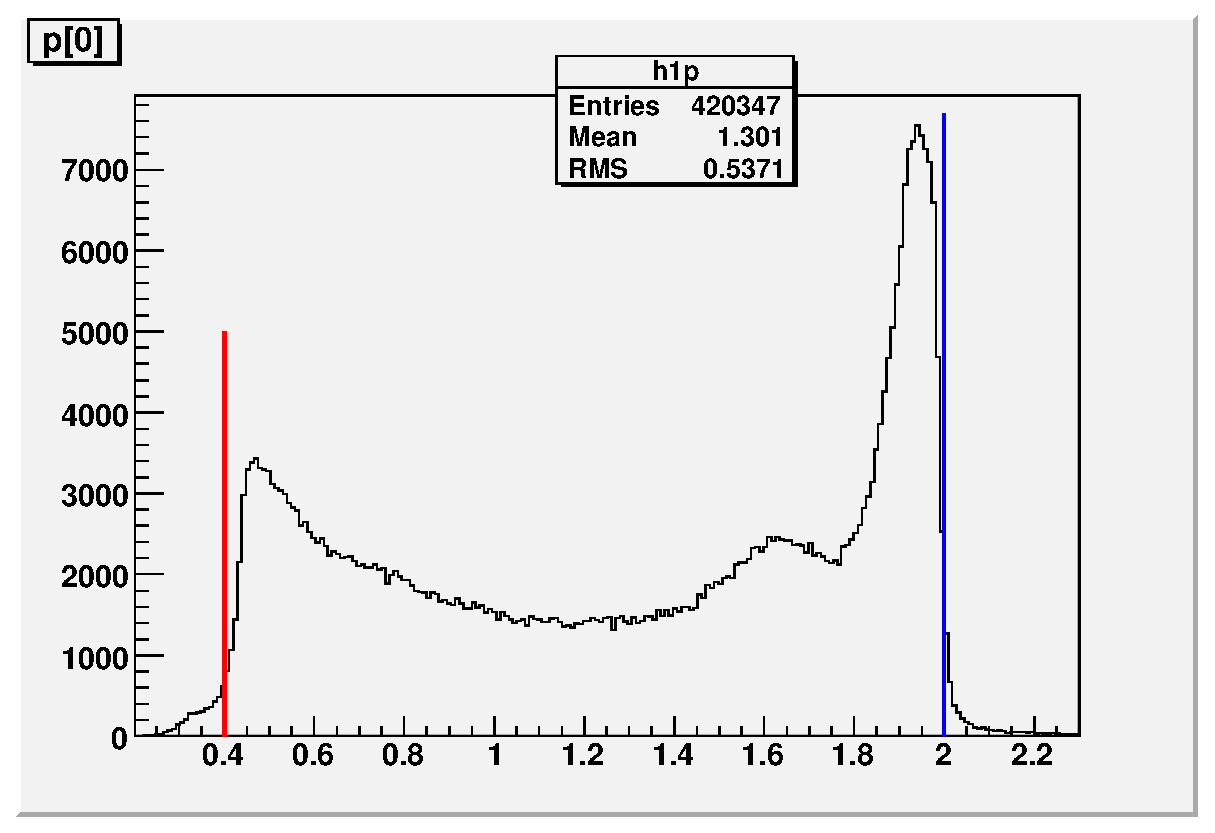
\includegraphics[width=0.8\textwidth]{TexmakerMyFinTh/chap4simul/FigCuts/pMinCtFrmRtPrmptEb2.eps}  %0.6 is the fraction of the real image width????
\leavevmode 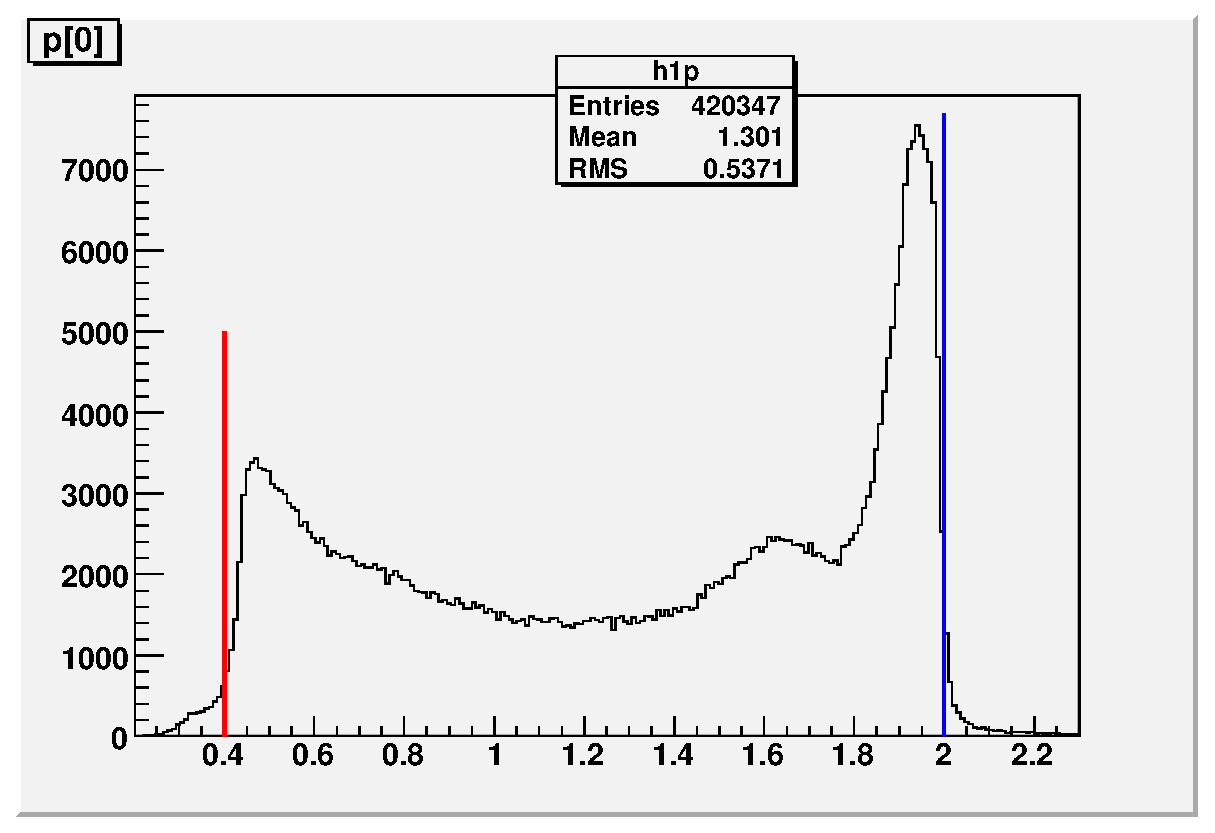
\includegraphics[width=0.8\textwidth]{TexmakerMyFinTh/chap4simul/FigCuts/pMinCtFrmRtPrmptEb2}  %0.6 is the fraction of the real image width????
\caption[Maximum and minimum momentum cuts]{The maximumum and minimum momentum cuts (on 2.0 GeV \nd3 data).
%\textcolor{red}{SEK: Memo to self: in the future use 0.45 GeV.}
}
\label{pMnMxCt}
\end{figure}

\subsection{Vertex-Z cuts}
\label{vzCuts}

In the EG4 experiment, the ND$_3$ polarized target was of 1 cm long and was placed at (x= 0, y = 0, z = -100.93 cm) in the CLAS coordinate system. Since the beam electrons have to go through a few foils %materials 
before reaching the target as well as the detector, 
we want to reject electron tracks with vertices 
%sometimes, many of the electrons that get detected happen to have scattered from points (scattering centers) that are outside the target volume. Our focus being on events that scattered off the actual target material, we want to reject those electrons that had %its 
%reconstructed vertices 
outside the target volume. %To do just that we 
For this purpose, use a cut on the reconstructed vertex co-ordinate ``v$_z$''. %But, because the resolution of ``v$_z$'' or any of the other variables is not good enough to cut events right at the edges of the target volum. Rather, the actual resolution
However the vertex resolution demands reasonably %much 
wide ``v$_z$'' cuts so as not to lose too many %much of 
good events. % due to the cuts applied. 
That is why the distribution of ``v$_z$'' was %is 
studied and based on the position and width of the distribution as well as our knowledge of the location of various foils and target materials, the cuts on ``v$_z$'' were decided. %Obviously, we were initially tempted to have a simpler, single set of cuts for all the kinematics (such as $\pm$ 4 or 5 cm on both sides of the nominal target  position), but it 
It was seen (see Figs. \ref{vzCtExp} and \ref{vzCtSim}) that the resolutions get worse and the distributions get wider as we go to lower \qsqs values, so again \qsqs dependent cuts were chosen for both data and simulation with the cuts tightening as \qsq increases.

\begin{figure}[H]%[htp] %ht, htpb (p - float, b = bottom, h=? t = top)
\centering
%\leavevmode 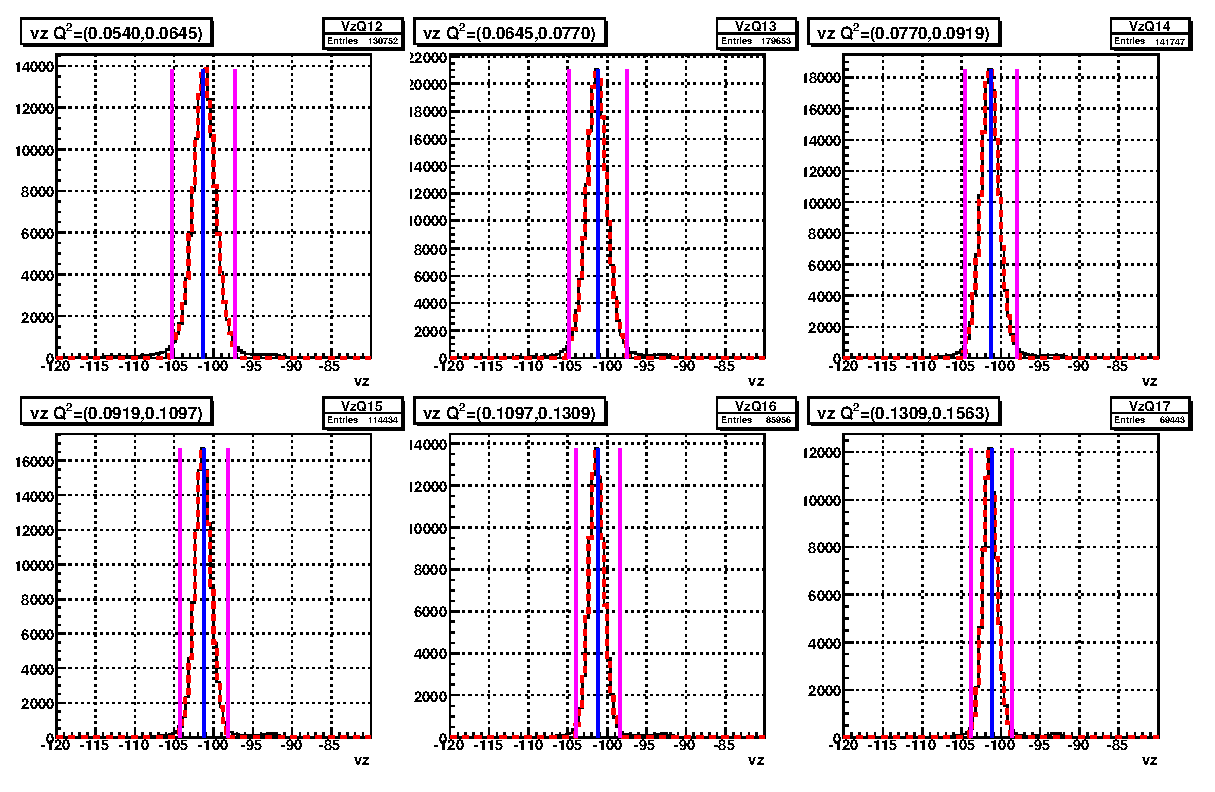
\includegraphics[width=1.0\textwidth]{TexmakerMyFinTh/chap4simul/FigCuts/vzCutsFinalEb2.eps}  %0.6 is the fraction of the real image width????
\leavevmode \includegraphics[width=1.0\textwidth]{TexmakerMyFinTh/chap4simul/FigCuts/vzCutsFinalEb2Ncropped}  %0.6 is the fraction of the real image width????
\caption[v$_z$ cuts (Exp.)]{2.0 GeV data showing the \qsqs dependent v$_z$-cuts (the magenta lines on the left and right of the peaks) in some of the \qsqs bins. The continuous black line represents events before applying all the other event selection cuts (except on v$_z$) and the thicker dotted red line are the events after the cuts. The blue lines are the centers of the distributions, from which the cuts are 3 times $\sigma$ away on each side, where $\sigma$ is the standard deviation for the distribution in the given \qsqs bin (both the central value and the $\sigma$ are determined during the cut development studies).}
\label{vzCtExp}
\end{figure}

As in the case of EC variables, the reconstructed ``v$_z$'' distribution in the simulation does not come out quite the same as in the experimental data %(see the separate section discussing the various issues encountered in simulation). Despite our tremendous efforts, intended agreement in the distributions could not be achieved and to 
. To have the same fraction of events in the corresponding \qsqs bins as in the experimental data, a separate set of cuts (determined based on the distributions of both types of data) had to be used for simulation. For this purpose, the Gaussian fit parameters $\mu$ and $\sigma$ (representing the mean and standard deviation) for all the \qsqs bins were tabulated separately for both data and simulation and separate sets of $\pm 3\sigma$ cuts were determined for all bins. For example, if $\mu_q$ and $\sigma_q$ were the two Gaussian fit parameters for the $q^{th}$ \qsqs bin of either data or simulation, then the lower and upper cuts for ``v$_z$'' for that data set in the given \qsqs bin would be $\mu_q - 3\sigma_q$ and $\mu_q + 3\sigma_q$ respectively (as shown by the magenta vertical lines in Figs. \ref{vzCtExp} and \ref{vzCtSim}.

%\textcolor{red}{My Original Question here was: Should I list all other cuts in a table (may go to Appendix)??}\\
%\textcolor{blue}{You wrote: ``Not sure what you mean''}\\
%\textcolor{red}{Because I showed these \qsq-dependent cuts for only 6 \qsqs bins (in figures), I was wondering if I should list the cuts for other bins in a table somewhere. I guess, may be not.}



\begin{figure}[H]%[h] %ht, htpb (p - float, b = bottom, h=? t = top)
%\leavevmode 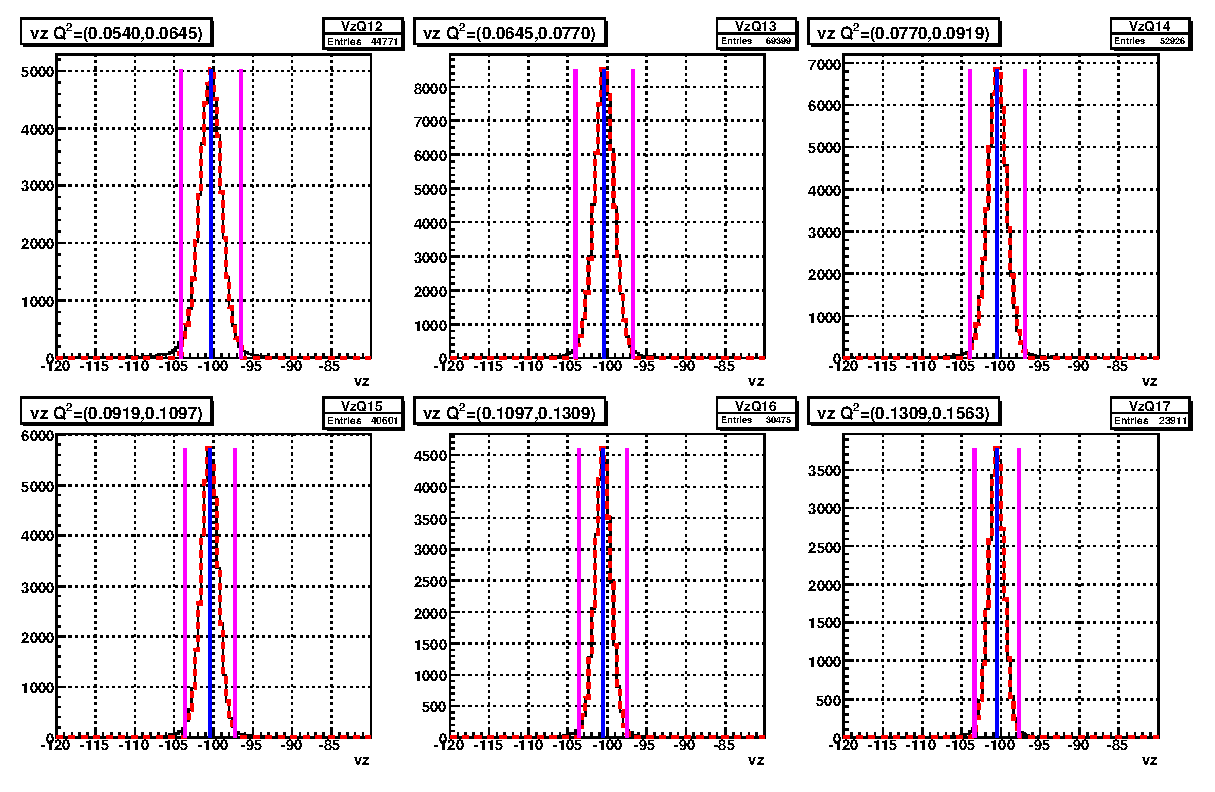
\includegraphics[width=1.0\textwidth]{TexmakerMyFinTh/chap4simul/FigCuts/vzCutsFinalEb2sim.eps}  %0.6 is the fraction of the real image width????
\leavevmode \includegraphics[width=1.0\textwidth]{TexmakerMyFinTh/chap4simul/FigCuts/vzCutsFinalEb2simNcropped}  %0.6 is the fraction of the real image width????
\caption[v$_z$ cuts (Sim.)]{\qsqs dependent v$_z$-cuts on simulation data (similar to Fig. \ref{vzCtExp}).}
\label{vzCtSim}
\end{figure}



%\section{Radiative Corrections}
%Plgiarism Warning: (paraphrasing not done.)
%GSIM - the CLAS Monte Carlo simulation program using GEANT 3.21 libraries from CERN -implements a complete. \cite{clasBrooks}%pg 31 

\subsection{Fiducial Cuts}
\label{fidCuts}

Similar to the cuts discussed so far, we also had to match the region of good efficiency of the physical detector with the corresponding region from the simulation. For the experimental and simulation data to be comparable, they must have the same detector acceptance. %, otherwise systematic uncertainty is introduced into the calculations. 
Two event variables polar angle (\thvtx) measured at the vertex and the azimuthal angle $\phi_{DC1}$ measured at the drift chamber layer 1 are chosen to define the good efficiency regions of the detector. The reason for the choice of the variable \thvtx~ should be obvious because it is directly related with the kinematic variables \qsqs and $W$ used in the analysis. However, due to the momentum dependent rotational effect of the magnetic field on the reconstructed azimuthal angle (\phvtx) at the vertex, the angle $\phi_{DC1}$ is preferred over \phvtx~ to define the fiducial region because that allows the easy selection (rejection) of the events which passed through and got detected by the more (less) reliable central (marginal) regions of the Cerenkov Counters. %drift chambers. %kp: 12/6/13 after SEK insistence
After a careful and extensive study of the event distributions on both data and simulation, we arrived at four sets of fiducial cuts in terms of the variables \thvtx, $\phi_{DC1}$ and the torus current normalized inverse momentum i.e., \invP.%I$_{torus}$/2250p.% This cut allowed the maximum possible inclusion of the high efficiency regions of

%
% Pass2 fiducial cuts: all defined in #include "/home/adhikari/LinkedFiles/fiducialCutsPass2.h"   
% The final results were for array indices C71 and S181
% The fiducial cuts used for C71_S181 were
%   
%
%   fidCtV1 
%   fidCtExpBySimAndEConlyInInvPvsThVtx
%   fidMoreMIPB
%
% %%%%%%%%%%%%%%%%  
%
%  where,
%   fidCtV1: if(fidCtExp2Sim==true && fidCtReg2EC==true) fidCtV1 = true;
%       with
%  bool fidCtReg2EC = Pass2FidCutLatestFromRegECcomparison(Ebi, p[0], thDc1PosRad);//now in the same fiducialCutsPass2.h file
%     corresponding image: 
%           https://www.jlab.org/Hall-B//secure/eg4/adhikari/Analysis/Pass2/Cuts/Fid/BkUp/invMomVsThDc1Pass2Ebi4Ratio.gif
%
%  bool fidCtExp2Sim = Pass2FidCutLatest(phDc1PosRad, thetaRadC); //now in the same fiducialCutsPass2.h file
%    corresponding image:
%          https://www.jlab.org/Hall-B//secure/eg4/adhikari/Analysis/Pass2/Cuts/Fid/fidCutPlotsSet2_Eb2_RatioBigger.gif 
%          &.../fidCutPlotsSet2_Eb1_Ratio.gif
%
%   
%
%   fidCtExpBySimAndEConlyInInvPvsThVtx = Pass2FidCutOnInvPvsThVtx(Ebi, ppC, thetaRadC);//3/8/16 defined in commonItems4SimExp.h for now
%              ~/secure/Analysis/Pass2/Cuts/Fid/invMomVsThVtxPass2Ebi1RatioRegByEConlyFidCut09.gif
%
%  if(Ebi==2) fidMoreMIPB = moreFidCutsWithMoreInvPBins(Ebi, ppC, phDc1DegPlusMinus30, thVtxDeg);//7/11/16 defined in moreFidCuts.h
%  else if(Ebi==1) fidMoreMIPB = moreFidCutsWithMoreInvPBinsEbi1(Ebi, ppC, phDc1DegPlusMinus30, thVtxDeg);//7/18/16 defined in moreFidCuts.h
%   for which see plots:
%       //https://www.jlab.org/Hall-B//secure/eg4/adhikari/Analysis/Pass2/Cuts/Fid/MoreCts/moreFiducialCutsMoreInversePBinsEbi1.gif
%       and moreFiducialCutsMoreInversePBinsEbi2.gif   //11/13/16
%   




% See EG4 update (Glasgow, by S.E. Kuhn) and make eps plots like those included
% include the DC shadow & granularity  figures, (may be in a separate section on Simulation/GSIM issues and refer to it from this section)

% include the Regular/EC-only 2D plots to show the CC-inefficient regions (to be discarded by some of the angular cuts)
% Show the discrepancy plots in theta and v$_z$ in data and simulation (for a few q2 bins)
%After a laborious work on getting simulation match with the data to a reasonably good degree, we did a final comparison work to determine the fiducial cuts. We obtained overlays of one-dimensional histograms of different variables, and also studied the ratios both in one and two dimensions. Based on these comparisons, regions of relatively bad matching were singled out and cuts were developed to reject such parts of the kinematic space.\textbf{\textcolor{red}{to be be elaborated more ..}}


The first set (see Fig. \ref{figFidRegVsEC1}) of fiducial cuts  were determined by comparing regular and EC-only data (which were taken using triggers that didn't involve CC) and selecting cuts such that regions with relatively darker spots (reflecting very low CC-efficiency) were rejected.

\begin{figure}[H]%[h] %ht, htpb (p - float, b = bottom, h=? t = top)
\centering
%\leavevmode \includegraphics[width=0.9\textwidth]{TexmakerMyFinTh/chap4simul/FigCuts/phDc1PosVsThv_inInvPbins_ExpEb2WdOsiNphNoThCts4Ths.eps} 
%\leavevmode \includegraphics[width=0.9\textwidth]{TexmakerMyFinTh/chap4simul/FigCuts/phDc1PosVsThv_inInvPbins_ExpEb2WdOsiNphNoThCts4Ths} 
%\leavevmode \includegraphics[width=0.9\textwidth]{figuresEG4/NewP2/FidCuts/invMomVsThDc1Pass2Ebi4Ratio.png}
%\leavevmode \includegraphics[width=0.9\textwidth]{figuresEG4/NewP2/FidCuts/invMomVsThDc1Pass2Ebi4RatioCropped.png}
%\caption[Fiducial cuts]{Fiducial cuts determined by comparing the distributions of regular and EC-only {\bf experimental data} as a function of \invP and $\theta_{DC1}$. %Here in the top panels, we see distributions of regular and EC-only data respectively and in the bottom panel we have the ratios of the two 
\leavevmode \includegraphics[width=1.0\textwidth]{figuresEG4/NewP2/FidCuts/invMomVsThVtxPass2Ebi4RatioCropped.png}
\caption[Fiducial cuts]{Fiducial cuts determined by comparing the distributions of regular and EC-only {\bf experimental data} as a function of \invP and $\theta_{vtx}$. %Here in the top panels, we see distributions of regular and EC-only data respectively and in the bottom panel we have the ratios of the two 
Here in the top panels, we see distributions of ratios of the regular and EC-only data respectively in linear and log scales in the color axis respectively. Inefficient regions of the CC are excluded using the indicated cuts.} %Fiducial cuts
\label{figFidRegVsEC1}
\end{figure}

The second set of cuts came from a similar comparison between the regular and EC-only data in the \invP vs \thvtx (instead of $\theta_{DC1}$) space (see Fig. \ref{figFidRegVsEC2}) .

\begin{figure}[H]%[h] %ht, htpb (p - float, b = bottom, h=? t = top)
\centering
%\leavevmode \includegraphics[width=0.9\textwidth]{TexmakerMyFinTh/chap4simul/FigCuts/phDc1PosVsThv_inInvPbins_ExpEb2WdOsiNphNoThCts4Ths.eps} 
%\leavevmode \includegraphics[width=0.9\textwidth]{TexmakerMyFinTh/chap4simul/FigCuts/phDc1PosVsThv_inInvPbins_ExpEb2WdOsiNphNoThCts4Ths} 
%\leavevmode \includegraphics[width=0.9\textwidth]{figuresEG4/NewP2/FidCuts/invMomVsThVtxPass2Ebi1RatioRegByEConlyFidCut09.png}
\leavevmode \includegraphics[width=0.9\textwidth]{figuresEG4/NewP2/FidCuts/invMomVsThVtxPass2Ebi1RatioRegByEConlyFidCut09cropped.png}
\caption[Fiducial cuts]{Fiducial cuts determined by comparing the distributions of regular and EC-only {\bf experimental data} as a function of \invP and vertex angle \thvtx. Here, the vertical cut near \thvtx=25 degrees is to avoid the region of low efficiency possibly due to %some dead wires
  dead wires in DC.} %Fiducial cuts
\label{figFidRegVsEC2}
\end{figure}



The third set of cuts came from a %somewhat similar
comparison %but this time 
between the experimental and the corresponding simulated data as shown in the Fig. \ref{figFidExpVsSim}. 
%The ratio of their distributions in a two dimensional space defined in terms of two variables \thvtx and the torus current normalized inverse momentum (i.e. $ I_{torus}/(2250 p)$. In one case, the ratio was taken between the regular experimental data and the "EC-only" experimental data (with CC-signal not required in the event trigger) (see Fig. \ref{figRegByEConly}) and in the other case, the ratio was of the experimental deuteron data (after background subtraction) to the simulated deuteron data (see Fig. \ref{figangCts2}). From these comparisons, some of the regions that showed big CC-inefficiencies or big discrepancies between data and simulation were selected and removed from the fiducial region %defined in terms of some more cuts 
as indicated by various straight lines in the two plots.



\begin{figure}[H]%[h] %ht, htpb (p - float, b = bottom, h=? t = top)
\centering
%\leavevmode \includegraphics[width=0.9\textwidth]{TexmakerMyFinTh/chap4simul/FigCuts/phDc1PosVsThv_inInvPbins_ExpEb2WdOsiNphNoThCts4Ths.eps} 
%\leavevmode \includegraphics[width=0.9\textwidth]{TexmakerMyFinTh/chap4simul/FigCuts/phDc1PosVsThv_inInvPbins_ExpEb2WdOsiNphNoThCts4Ths} 
%\leavevmode \includegraphics[width=0.98\textwidth]{figuresEG4/NewP2/FidCuts/fidCutPlotsSet2_Eb2_RatioBigger.png}
\leavevmode \includegraphics[width=0.98\textwidth]{figuresEG4/NewP2/FidCuts/fidCutPlotsSet2_Eb2_RatioBiggerCroppedIpBins0n1.png}
\caption[Fiducial cuts ]{Distribution (in two of six bins of $I_{torus}/(2250 p)$) of %{\bf experimental} and {\bf simulated} data ( for 2.0 GeV) and their ratios 
ratios of {\bf experimental} and {\bf simulated} data ( for 2.0 GeV) (both in linear and log-z scales) as a function of vertex angle $\theta_{vtx}$ and azimuthal angle $\phi_{DC1}$ as measured by the track position at the first drift chamber layer (angles in degrees). The dotted lines indicate the fiducial cuts for accepting good electrons. %\textcolor{red}{SEK: Do you have the analogous plot for simulation? Include \\ Make magenta lines thicker. } %Comment out eventually
} %Fiducial cuts}
\label{figFidExpVsSim}
\end{figure}


%> 1) Fiducial cuts (Very short)   %Dr. Kuhn's comment on Jlab email dated November 3, 2013 3:45 pm  (title Re: "Complete" Thesis)
%
%p. 116: We used the polar angle at the vertex NOT because it isn't affected by the target magnetic field (it most certainly is), but because the acceptance is defined by the range in scattering angle (as you showed earlier, dOm = sintheta dtheta dphi). For the same reason, we SHOULD have chosen phi at the vertex, as well; however, since the effect of the target field on phi is just a constant offset (rotation around the z-axis), the range phi_max - phi_min is the same at DC1 as at the vertex, giving the same acceptance. We chose DC1 because that's what actually limits the phi acceptance. As you understand, this section is not yet complete. You need to explain that we use the amount of bending (Itor/p*2250) as a 3rd variable, since E'=p is the third variable the determines the acceptance, but the amount of bending has direct correlation to where on the CC a track ends (i.e., the phi range). (You should move the corresponding explanation of ip up from p.122).                      You should also show a couple more plots with different Itor/p*2250 as well as a couple of plots for the simulation to convince the reader that our choices are robust.                   Figs. 51a and 51b should be given a full width each since they have a lot of information and are hard to read otherwise (make them two different figures). I also am confused about your explanation for Fig. 51a):                  I seem to remember that we divided ND3 for standard trigger by ND3 for EC only trigger;  dividing ND3 data by D simulation seems to make little sense. Please check!

Lastly, further sets of cuts were developed based on the distribution of the average number of photo electrons (nphe) as recorded by the Cerenkov Counter (CC) (see Fig. \ref{figFidAvgNph1}).

\begin{comment}
\begin{figure}[H]%[h] %ht, htpb (p - float, b = bottom, h=? t = top)
\centering
\leavevmode \includegraphics[width=1.1\textwidth]{figuresEG4/NewP2/FidCuts/moreFiducialCutsMoreInversePBinsEbi2.png}
\caption[Fiducial cuts ]{}
\label{figFidAvgNph}
\end{figure}
\end{comment}


\begin{figure}[H]%[h] %ht, htpb (p - float, b = bottom, h=? t = top)
\centering
%\leavevmode \includegraphics[width=1.1\textwidth]{figuresEG4/NewP2/FidCuts/moreFiducialCutsMoreInversePBinsEbi2first4Bins.png}
\leavevmode \includegraphics[width=1.1\textwidth]{figuresEG4/NewP2/FidCuts/moreFiducialCutsMoreInversePBinsEbi2first4BinsN.png}
\caption[Fiducial cuts (first 4 bins)]{Average Nphe distributions as a function of $\phi_{DC1}$ (along Y-axis) and $\theta_{vtx}$ (along X-axis) in first four bins of $\frac{I_{tor}}{p \cdot 2250}$. The black lines show the cuts that reject the very low CC-inefficiency regions.}
\label{figFidAvgNph1}
\end{figure}


\begin{figure}[H]%[h] %ht, htpb (p - float, b = bottom, h=? t = top)
\centering
\leavevmode \includegraphics[width=1.1\textwidth]{figuresEG4/NewP2/FidCuts/moreFiducialCutsMoreInversePBinsEbi2next4Bins.png}
\caption[Fiducial cuts (next 4 bins)]{Average Nphe distributions as a function of $\phi_{DC1}$ (along Y-axis) and $\theta_{vtx}$ (along X-axis) in next four bins of $\frac{I_{tor}}{p \cdot 2250}$. The black lines show the cuts that reject the very low CC-inefficiency regions.}
\label{figFidAvgNph1}
\end{figure}


\begin{figure}[H]%[h] %ht, htpb (p - float, b = bottom, h=? t = top)
\centering
%\leavevmode \includegraphics[width=1.1\textwidth]{figuresEG4/NewP2/FidCuts/moreFiducialCutsMoreInversePBinsEbi2last4BinsN.png}
\leavevmode \includegraphics[width=1.1\textwidth]{figuresEG4/NewP2/FidCuts/moreFiducialCutsMoreInversePBinsEbi2last4BinsN.png}
\caption[Fiducial cuts (last 4 bins)]{Average Nphe  distributions as a function of $\phi_{DC1}$ (along Y-axis) and $\theta_{vtx}$ (along X-axis) in last four bins of $\frac{I_{tor}}{p \cdot 2250}$. The black lines show the cuts that reject the very low CC-inefficiency regions.}
\label{figFidAvgNph1}
\end{figure}


%%%%%% To be worked 
%%%%%% To be worked 
%%%%%% To be worked 
%%%%%% To be worked 
%%%%%% To be worked 



\clearpage
